\documentclass[12pt]{article}
\usepackage[utf8]{inputenc}
\usepackage{amsmath}
\usepackage{graphicx}
\graphicspath{ {images/} }
\usepackage[colorinlistoftodos]{todonotes}

\usepackage{float}
\usepackage{wrapfig}
\usepackage{float,subcaption, geometry}
\usepackage[rightcaption]{sidecap}
\usepackage[export]{adjustbox}

% Plotting package
\usepackage{pgfplots}
\pgfplotsset{width=10cm,compat=1.9}
\usepackage{pgf-pie}

% references
\usepackage[
backend=biber,
style=alphabetic,
citestyle=authoryear-comp 
]{biblatex}
 
\addbibresource{cs4099_bib.bib}     %imports bib file

% hyper ref
\usepackage{hyperref}
\hypersetup{
    colorlinks,
    citecolor=black,
    filecolor=black,
    linkcolor=black,
    urlcolor=black
}

% Javascript / JQuery Code listing
\usepackage{textcomp}
\usepackage{listings}
\usepackage{color}

\lstdefinelanguage{JavaScript}{
        keywords={typeof, new, true, false, catch, function, return, null, catch, switch, var, if, in, while, do, else, case, break},
        keywordstyle=\color{blue}\bfseries,
        ndkeywords={class, export, boolean, throw, implements, import, this},
        ndkeywordstyle=\color{darkgray}\bfseries,
        identifierstyle=\color{black},
        sensitive=false,
        comment=[l]{//},
        morecomment=[s]{/*}{*/},
        commentstyle=\color{purple}\ttfamily,
        stringstyle=\color{red}\ttfamily,
        morestring=[b]',
        morestring=[b]"}

\lstset{
  language=JavaScript,
   backgroundcolor=\color{lightgray},
   extendedchars=true,
   basicstyle=\footnotesize\ttfamily,
   showstringspaces=false,
   showspaces=false,
   numbers=left,
   numberstyle=\footnotesize,
   numbersep=9pt,
   tabsize=2,
   breaklines=true,
   showtabs=false,
   captionpos=b
}

% header
\usepackage{fancyhdr}
\pagestyle{fancy}
\fancyhf{}
\rhead{Michael Sime}
\lhead{CS4099 Senior Honour Project}
\cfoot{\thepage}

\begin{document}

\begin{titlepage}

\newcommand{\HRule}{\rule{\linewidth}{0.5mm}} % Defines a new command for the horizontal lines, change thickness here

\center % Center everything on the page

%-------------------------------------------------------------------------------------
%	TITLE SECTION
%-------------------------------------------------------------------------------------

\HRule \\[0.4cm]
{ \Huge \bfseries An Analysis of the Mechanisms and Techniques used in web-based Targeted Advertising and an Implementation of an IFrame Ad-Explorer}\\
\HRule \\[1.5cm]


%-------------------------------------------------------------------------------------
%	LOGO SECTION
%-------------------------------------------------------------------------------------

\adjincludegraphics[height=9cm,trim={0 {.1\width} 0 {.25\width}},clip]{university_logo.png}\\
 

%-------------------------------------------------------------------------------------
%	HEADING SECTIONS
%-------------------------------------------------------------------------------------

\textsc{\Large CS4099: Senior Honours Project}\\[1cm]

%-------------------------------------------------------------------------------------
%	AUTHOR SECTION
%-------------------------------------------------------------------------------------

\begin{minipage}{0.4\textwidth}
\begin{flushleft} \large
\emph{Author:}\\
Michael \textsc{Sime} % Your name
\end{flushleft}
\end{minipage}
~
\begin{minipage}{0.4\textwidth}
\begin{flushright} \large
\emph{Supervisor:} \\
Colin \textsc{Allison} % Supervisor's Name
\end{flushright}
\end{minipage}\\ [0.75cm]


%-------------------------------------------------------------------------------------
%	DATE SECTION
%-------------------------------------------------------------------------------------

\textsc{Date of submission: April 4 2016}\\

\vfill % Fill the rest of the page with whitespace

\end{titlepage}

\pagestyle{plain}
\begin{abstract}
The innovation of the world wide web has spawned completely new forms of marketing and advertising. The most prevalent and insidious of these  is targeted advertising. The contemporary network of entities that interact to profile and track individuals whilst  bidding for and placing adverts within a website in real time is complex and lacks transparency. This project will delve into the mechanisms and techniques used by organisations to i) profile individuals; ii) identify them when they are web browsing; iii) create and display targeted adverts to users in real time. It will also i) discuss methodologies and tools designed to reduce the effectiveness of such advertising;  ii) create a framework of tools and methods to help improve the transparency of web tracking and profiling to the end user; iii) investigate the various forms of digital advertising fraud.  
\end{abstract}

\section{Declaration}
I declare that the material submitted for assessment is my own work except where credit is explicitly
given to others by citation or acknowledgement. This work was performed during the current academic year
except where otherwise stated. The main text of this project report is 19,723 words long,
including project specification and plan. In submitting this project report to the University of St
Andrews, I give permission for it to be made available for use in accordance with the regulations of the
University Library. I also give permission for the title and abstract to be published and for copies of the report to be made and supplied at cost to any bona fide library or research worker, and to be made available on the World Wide Web. I retain the copyright in this work.

\pagebreak

\tableofcontents

\pagebreak

\pagestyle{fancy}
\section{Introduction}
Online advertising has existed since the inception of the World Wide Web. The first clickable advert, which was later defined as a banner ad, was sold on the web by Global Network Navigator in 1993 to Heller, Ehrman, White, \& McAuliffe, a law practice in Silicon Valley \parencite{oreilly}. The first mass production of advertising was implemented by \textit{HotWired.com} (now called Wired) which sold a large number of banner ads to corporate advertisers \parencite{firstAd}. These organisations were at the cutting edge of advertising which has subsequently spawned into the complex ecosystem that online advertising is today. Online advertising is an increasingly broad category which takes up a large percentage of advertising budgets worldwide. The forecasts of Statistia state that digital advertising spending increased to approximately \$146 billion in 2015 and is expected to reach \$252 billion by 2018 \parencite{Statistia}. Figure \ref{fig:M1} shows the upward trend in spending on online advertising which looks likely to become the most common form of advertising.   \\

\begin{figure} [H]
    \centering
    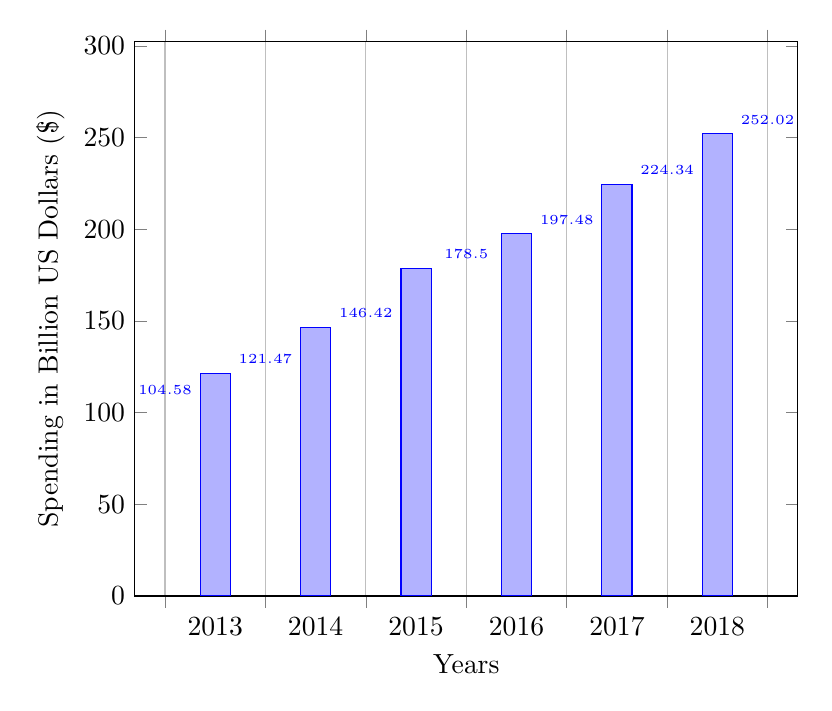
\begin{tikzpicture}
        \begin{axis}[
        	x tick label style={
        		/pgf/number format/1000 sep=},
        	ylabel= Spending in Billion US Dollars (\$),
        	xlabel= Years,
        	enlargelimits=0.05,
        	enlarge y limits={value=0.2,upper},
        	legend style={at={(0.5,-0.1)},
        	anchor=north,legend columns=-1},
        	ybar interval=0.3,
        	ymin=0,
        	nodes near coords,
        	every node near coord/.append style={font=\tiny},
        	nodes near coords align={vertical}
        ]
        \addplot 
        	coordinates {(2018, 252.02) (2017, 224.34) (2016, 197.48) (2015, 178.50) (2014, 146.42) (2013,121.47) (2012,104.58)};
        \end{axis}
    \end{tikzpicture}
    \caption{Results and forecasts of global online advertising spending \parencite{Statistia}.} \label{fig:M1}
\end{figure}


The Federal Trade Commission (FTC) defines targeted advertising as ``the practice of tracking an individual’s online activities in order to deliver advertising tailored to the individual’s interests'' \parencite{comission2009}. Targeted advertising is a controversial topic, as 68\% of Internet users surveyed disapproved of search engines and websites tracking their online behaviour for the purpose of tailoring adverts to them \parencite{usersTA}. Furthermore, an additional survey found that only 6\% of users were aware of the Digital Ad Alliance's AdChoices privacy icon, a small blue triangle, which is primarily shown alongside targeted advertising. This allows users to opt-out from specific adverts \parencite{AdChoices}. In contrast to the lack of widespread knowledge of opt-out programs, research showed that 87\% of users surveyed are in favour of a ``Do Not Track" button which would prevent advertisers from gaining access to online purchasing and visiting history \parencite{dnt87}. Despite this strong stance on tracking, research has also illustrated consumers are willing to trade their data for benefits such as discounts on products. Younger generations are more willing to do this than older generations as 60\% of Millennials would voluntarily share their information for discounts or promotions while only 38\% of the Silent Generation are willing to do so \parencite{dnt87}. Along with this when asked whether they would prefer to see online adverts for random products and services or adverts directed toward their interests, 40.5\% of respondents chose targeted adverts, with 27.6\% of respondents stating they were comfortable with seeing both type of adverts \parencite{randomAds}. Moreover, 47.3\% of respondents would oppose a law that ``restricted how data is used for online advertising, but also potentially reduced the availability of free content such as blogs and video sites.” \parencite{randomAds}. This is most likely due to a reduction in free content, as 9 in 10 respondents said that free content like news, weather, email, blogs and videos was extremely or somewhat important to their overall value of the Internet. \\

These various statistics show the diverse range of consumer opinion on the topic of targeted advertising, whilst some view it as an invasion of their privacy, others see it as a price to pay to access the wealth of free content on webpages funded by advertising. Previous studies have stressed the privacy concerns about targeted adverting, proposing a privacy enhancing framework \parencite{wang2015privacy}, whilst others analysed the effectiveness of targeted advertising \parencite{brahim2011targeted}. This paper will focus upon the techniques used by  advertisers to create tailored online behavioural advertising. \\

The online advertising industry is a secretive and poorly documented area. The major objective of this project is to expose the area of targeted advertising, educating them on the practises used by trackers to profile users whilst providing advice on how to improve their privacy. The project will seek to bring the methods used to track and create profiles of users to the forefront, whilst creating a framework of tools to expose the source of IFrame adverts on webpages, it also discusses the contemporary issues of ``Ad Blocking" and online advertising fraud. The project has met all of the aims set out for it in Section \ref{requirements}, consolidating previous research and producing novel research which will be of benefit to all users of the Internet. The covert nature of the online advertising industry combined with the lack of documentation surrounding its processes and procedures meant a disproportionate amount of time during this project was spent researching and understanding the area before a deliverable could be designed. This complication limited the amount of time spent on the development of the software deliverable of the project. However, the deliverable was finished and in future work it would merely require a final User Interface (UI) polish before it could reach its full potential.   \\

The following sections of the report explore the domain of targeted advertising from a technological perspective: discussing the entities involved and how they interact with one another, examining the tools used by organisations to track and profile users, defences users can employ to limit the effectiveness of these tracking mechanisms, the contentious area of Ad Blocking and a discussion of how fraud is affecting the online advertising industry. This report has centralised a large amount of information from the broad area of targeted advertising. There are numerous terms and acronyms used within the industry which have been summarised in the glossary of Appendix D in Section \ref{glossary}. After these areas have been discussed the project requirements are detailed. The framework of IFrame Ad-Exploring tools is then presented from a software engineering perspective, beginning with the design of the system through to the testing and future improvements that could be made to the system. Finally the success of the project is evaluated and it is put in perspective of other work in the targeted advertising field, this includes a discussion of the future of user tracking and profiling.  

\pagebreak

\section{Entities involved in Targeted Advertising} 
There are numerous entities involved in targeted advertising such as the Advertiser, the Demand Side Platform (DSP), the Supply Side Platform (SSP), Ad Networks and Ad Exchanges, and the Publisher. An advertiser and a publisher are normally connected by an Ad Network which has a large amount of advertising infrastructure and for a fee will facilitate its services e.g. \textit{Google AdSense}. This is discussed in more detail in Section \ref{AdNetwork}. The parties can also be connected by an Ad Exchange as discussed in Section \ref{AdExchanges}. Parties wishing to advertise can also utilise Demand Side Platforms to purchase digital advertising inventory this is discussed in Section \ref{DSP}. In contrast to DSPs, Supply Side Platforms can be utilised by web publishers to manage their advertising space inventory, filling it with adverts and receiving the corresponding revenue. This platform will be discussed in Section \ref{SSP}. A high level process diagram of the current interactions between these entities is shown in Figure \ref{fig:ta_process}. Along with the digital advertising sector the interactions between these units is frequently evolving as new processes are developed and entities attempt to amalgamate processes into one centralised system.

\begin{figure}[H]
    \centering
    \includegraphics[width=1\textwidth]{ta_process}
    \caption{An overview of the relationships between the targeted advertising entities}
    \label{fig:ta_process}
\end{figure}

\subsection{Advertiser}
In the context of online advertising, the advertiser is an entity which has a product that they wish to promote and are willing to pay for this promotion on a website e.g. \textit{Coca-Cola}.

\subsection{Publisher} 
The publisher in this case is any website that is willing to give up real-estate on their page for an Advertiser's product e.g. \textit{theguardian.com}.

\subsection{Ad Networks} \label{AdNetwork}
Online Ad Networks began to appear in 1997. The original Ad Networks were created to address the problem of advertisers wanting to buy online inventory \parencite{adExchanges}. Internet audiences are incredibly fragmented, splitting their online time between many different websites. This is in contrast to the traditional forms of media such as print, radio and television. By aggregating inventory across multiple sites, Ad Networks could offer advertisers the ability to reach the size of audience that they had come to expect from traditional channels of advertising. \newline

Ad Networks can be defined as a company that connects advertisers to web sites that want to host advertisements. The key function of these networks is aggregation of Ad space supply from publishers and matching it with advertiser demand. 

\subsection{Ad Server}
An Ad Server is defined as the technology and services that places an advertisement upon a website. This technology can also be used to count the adverts, select more profitable locations for adverts and monitor the progress of different advertising campaigns. Ad Servers can be categorised into two types: Publisher Ad Servers and Advertiser or Third Party Ad Servers. \newline 

Typically an Ad Server is a web server backed by a database server which can be used to store the advertisements and delivers them to website visitors. The contents of the web server are constantly updated so that the website which is used to display the ads contains fresh advertisements. The aim of Ad serving is to deliver the content of adverts to users by placing adverts on the publisher's web page, to manage a websites advertising space and in the case of Advertiser Ad Servers to provide an independent counting and tracking system to advertisers. \newline 

When Ad Servers are run locally by a single publisher they can be used to serve ads to that publisher's domain, allowing fine-grained, creative, formatting and content control by that publisher. However, remote Ad Servers can serve Ads across domains owned by multiple publishers. This one centralised repository of adverts can allow advertisers and publishers to track the distribution of their online advertisements. 

\subsection{Demand Side Platform} \label{DSP}
The Demand Side Platform (DSP) can be described as software used to purchase advertising in an automated fashion. DSP facilitates a buyer with direct Real Time Bidding (RTB) access across multiple sources of inventory \parencite{introDSP}. Advertisers use DSPs to purchase impressions (an advertising slot) across a range of publisher sites, but targeted to specific users based on information such as their location and previous browsing history. Thus, enabling buyers to access a wider range of publishers and select the most appropriate for their requirements. For example Apple might recognise that a user has previously been on their site looking at a specific computer and therefore they may be prepared to pay more than Amazon or EasyJet to serve ads to the user. This process removed the human element of digital advertising which in turn improved the efficiency of the process whilst reducing the costs via automation. Publishers will make their impressions available through marketplaces called Ad Exchanges, discussed in Section \ref{AdExchanges}, and then DSPs will automatically decide which impressions suit the requirements of the advertiser and purchase these impressions. Demand Side Platforms are offered by a large number of companies for example: App Nexus, Google DoubleClick, AdForm. 

\subsection{Supply Side Platform} \label{SSP}
A Supply Side Platform (SSP) is the publisher's equivalent of a DSP. Where DSPs are utilised by advertisers to buy ad impressions from exchanges in the most cost effective and efficient manner possible, SSPs are designed by publishers to do the opposite: to maximise the price an impression sells at. SSPs allow publishers to connect their inventory to multiple Ad Exchanges, DSPs and Ad Networks at once. This increases the range of potential buyers dramatically which in turn can force the price of impressions higher and ensure that publishers get the highest possible rates therefore maximising the revenues they receive for their inventory. Whenever a Supply Side Platform is used to place an impression into various Ad Exchanges, DSPs will analyse and purchase them on behalf of marketers depending on attributes such as where they are served on the screen and which specific users they're being served to \parencite{introDSP}. Example of SSPs are: AppNexus Publisher Suite, Yahoo and OpenX SSP.  

\subsection{Real Time Bidding}
Real Time Bidding (RTB) is a deterministic process by which advertising inventory is bought and sold on a per-impression basis, via programmatic instantaneous auction, this approach is analogous to the financial markets \parencite{RTB}. With RTB advertising buyers bid on an impression in a real-time auction that occurs in the time it takes a web page to load. If the bid is won, the buyer's ad is instantly displayed on the publisher's site. These auctions are often facilitated by Ad Exchanges or Supply Side Platforms. One of the main advantages of Real Time Bidding is that it facilitates advertisers to manage and optimise adverts from multiple Ad Networks by granting the user access to a multitude of different networks. Furthermore it gives advertisers the ability to create advertising campaigns on an instantaneous basis and allocate a much higher percentage of their unsold advertising inventory. \newline

In its simplest form, the RTB process unfolds much like the following: 
\begin{enumerate}
\item The publisher provides its inventory to an Ad Exchange, who is responsible for holding an auction, during which the DSPs, on behalf of the advertisers, will place a bid on each impression \parencite{howRTBWorks}. 
\item The value of the bid is based on the expected value of that impression to the advertiser based upon the parameters they have passed to the DSP. The auction process ensures that each impression is sold at as high a price as possible as dictated by the demand in the real-time market \parencite{howRTBWorks}. 
\item Once the bidding is over, the winner is chosen and their ad is served on the publisher's website. 
\end{enumerate}

\subsection{Data Management Platform}
To acquire the large amounts of data needed to target and potentially re-target users with advertisements many organisations now use Data Management Platforms (DMP). DMPs are essentially a data warehouse, a piece of software that is utilised to store, sort and report on the vast amount of data used by all businesses involved with the programmatic advertising process. In a similar manner to a database DMPs can be used to house and manage any form of information but marketers most often utilise the platform to manage cookie IDs and to generate audience segments, which are subsequently used to target specific users with online adverts \parencite{DMP}. As previously discussed the myriad of middlemen including DSPs, Ad Networks and exchanges makes it hard for advertisers to keep track of their performance. Therefore, a Data Management Platform can be used as a centralised repository to keep all audience data and resulting performance of advertising together, which allows advertisers to optimise future inventory purchasing and Ad creativity. Examples of Data Management Platforms include: Oracle DMP (powered by BlueKai), Adobe Audience Manager and Krux. \newline

DMPs can be used on both sides of the advertising ecosystem. Information can be fed from a marketer's DMP to its DSP to help inform Ad purchasing decisions, but without being linked to another technology, a DMP is largely redundant. In contrast, DMPs can be 
utilised by publishers by linking them to a SSP. In this case, the DMP holds publisher information on its readers, which may help them to sell their adverts for a higher price. Like many of the areas discussed in this paper the line between DMPs and DSPs are largely artificial and are beginning to blur, as growing number of DSP providers now offer their clients DMP services too.  

\subsection{Ad Exchanges} \label{AdExchanges}
Ad Exchanges can be seen as the medium through which Ad impressions from publishers can be made available to potential buyers. An advert exchange is a technology platform that facilitates the buying and selling of media advertising inventory whose prices are determined through an online auction with bidding coming from multiple Ad Networks, this process is also referred to as Real Time Bidding. This approach is technology-driven as opposed to the traditional process of negotiating prices on media inventory in advance. Examples of these platforms are: DoubleClick, AdECN, Rubicon Project and Open X. \newline

\begin{figure}[H]
    \centering
    \includegraphics[width=1\textwidth]{adExchange}
    \caption{An example interaction on an Ad Exchange platform \parencite{adExchanges}}
    \label{fig:adExchange}
\end{figure}

Whenever a user visits a website, in the short interval of the page load time, in the background an Ad Exchange conducts an auction between multiple advertisers for each impression on that page. The advertisers bid for the impression of the user and compare this to their target behavioural and demographic profile, along with the subject matter of the website and the dimensions of the ad (including placement on the site). The highest bidder during the auction will win the right to place an ad on the website. This whole procedure takes place in ``real-time'' in the short number of milliseconds it takes for a web page to load, an example of the auction process is illustrated in Figure \ref{fig:adExchange}. 

\subsection{ Targeted Ad Networks}
Targeted Ad Networks differ from an Ad Network by allowing advertisers to buy audience segments such as: demographics (e.g. gender, age),  behavioural segments (e.g. interest in buying a home), by context (e.g. websites that are in a particular subject area) or by alternatives to Cost Per Mille (CPM), a definition of this term can be found in the glossary in Section \ref{cpm}, such as cost per 100 viewers of the advertisement. This holds a significant advantage for advertisers as it offers them the ability to buy on a performance basis. Similarly, this structure offers benefits to publishers who have the ability to sell remnant inventory without cannibalizing higher priced inventory sold directly via Ad Networks \parencite{adExchanges}. Examples of Targeted advertising networks include: Google AdSense, Yahoo! Publisher network and AOL Advertising.

\pagebreak

\section{User Profiling}
As the prevalence of online advertising has increased, the techniques to identify users based on their web browsing and purchase history have developed in tandem with this dramatic rise. This section details the most pervasive techniques for tracking users, discussing how they profile users, how effective they are and how pervasive they are. This section is split into two subsections: stateful and stateless tracking mechanisms. A stateful tracking method will store a uniquely identifiable file connected to a user on the storage of their computer. In contrast to this stateless tracking mechanisms do not have to store a file, they rely on the characteristics of the user's browser or features of the protocols utilised when making requests to web servers.

\subsection{Stateful Tracking Mechanisms}

\subsubsection {Cookies} \label{cookies}
A cookie can be defined as a triple (domain, key, value) that is stored in the browser across page visits, where the domain is a particular website and the key and value are opaque identifiers \parencite{roesner}. The cookie mechanism adds state to the otherwise stateless HTTP protocol, as the cookies allow a web server to store a small amount of data \footnote{approximately 4 Kilobytes (KB)} on the computers of the visiting users which is then sent back to the web server upon subsequent requests \parencite{cookielessMonster}. The information contained in the cookie could be about the user's previous browsing activity such as logging in, clicking particular buttons and sites they have previously visited or it could contain stateful information for example what items they added to their shopping cart. Although, the most controversial cookies are those that are utilised to manage the advertising on a website, these cookies can be set from a separate advertising delivery company. A cookie of this type can record when and where a user saw an advert and whether they chose to click through the advert to purchase the product. This information will then be returned to the cookie owner who records the data and will use that to inform behavioural targeting for future adverts placed in front of a user.  \newline 

There are two types of cookies \textit{first-party} and \textit{third-party}. First-party cookies are set by the domain that the user visits directly, i.e. the domain in the address bar, for example, if a user visits www.google.com then cookies that are set with the domain of www.google.com are first party cookies. Third-party cookies are set by a different domain than the one the user visits, they are embedded in the top-level page, for example if a visitor visits www.amazon.com and the domain of the cookies added are www.google.com then these cookies are third-party cookies. \newline

There are numerous ways cookies can get to a webpage. Traditionally cookies were set by using an HTTP response that included a Set-cookie header, however cookies can appear in a browser in a numerous more subtle methods now. They can be set either by Javascript scripts running in the page or by using an API call from within a plug-in. Cookies are one of the simplest yet most effective ways to gain information about a user which can then be used for behavioural targeted advertising, or to build a profile about a user to place them in an audience segment. As the information in the cookie is constantly evolving dynamically with user actions it is very effective for trackers to place a cookie within a user's browser. 

% TODO: research this
\subsubsection{Supercookies} \label{Supercookies}
The term supercookie is used to refer to methods utilised to uniquely identify users that do not rely on HTTP cookies. A supercookie generally refers to a means of storing something unique from a website on a user's computer so that it can be retrieved the next time the user visits that website. The name is rather misleading as these methods of tracking aren't technically cookies as they are not placed on a user's computer via the HTTP protocol. \newline 

Local Shared Objects (LSOs) found within the Adobe Flash plugin are used to provide Flash applications with the ability to save options to the local system, for example, to save progress in a game. But as there is not a distinction between good and bad usage of this mechanism many websites have began to save persistent information on the user system as an alternative to third-party HTTP cookies. The output from this exploit is referred to as a ``Flash cookie", as a tracking organisation could use this method to place uniquely identifiable data directly on a user's computer. Flash cookies are still a frequently used resource in the domain of tracking as a user cannot access them easily from within the browser. Flash cookies are not located with other HTTP cookies, easily accessible from a cookie manager in the browser, nor are they present in databases or other browser-specific storage locations \parencite{flashCookies}. A user must also travel to the Adobe Flash Player Settings Manager webpage (\url{http://www.macromedia.com/support/documentation/en/flashplayer/help/settings_manager07.html}) to manage or delete Flash cookies and update their related settings, which is both unintuitive and poorly documented. Therefore users who have cleared their HTTP cookies may think they are no longer being tracked, however websites utilising LSOs will still be able to track them. This process is not transparent to the user meaning that they can be unaware they are still being tracked.\\ 

Another reason, why they are potentially favoured in a tracking context is that traditional HTTP cookies are limited in size to 4 Kilobytes of data whereas Flash cookies can be utilised to store up to 100 Kilobytes \parencite{flashCookies}. The larger storage capacity and difficulty in removing Flash cookies makes them an effective means of tracking even a privacy conscious user. Although the evolution of HTML5 has limited the appeal of Adobe's Flash browser plugin it still commands usage on 9.3\% of Internet sites compared with 2010 where 28.5\% of global Internet sites used the platform \parencite{flashStats}. Adobe reports that there are more than 500 million devices addressable with Flash technology, and this is projected to increase to over 1 billion addressable devices by the end of 2015 \parencite{adobeFlash}. These statistics illustrate that although adoption rates of Flash may be slowing the Flash cookie method of tracking is still relevant and could be used to profile a large number of users, most of which would unaware they were being tracked. 

% TODO: add more?
\subsubsection{Evercookies} \label{evercookies}
An evercookie is a specialisation of a supercookie, it is a resilient tracking mechanisms that uses multiple storage vectors including Flash cookies, localStorage, sessionStorage and ETags \parencite{evercookies}. Evercookies use this information to identify a client even after they've removed standard cookies. This is similar to the ``re-spawning" of cookies shown in \parencite{flashCookiesPrivacy} which illustrated the abuse of Flash cookies for regenerating previously removed HTTP cookies. The rationale behind the evercookie API is to make stateful methods of tracking persistent. By storing the same data in a multitude of storage locations, if any tracking information is lost or removed it can simply be recovered from another storage location and then continue to be used for tracking purposes. At the time of writing this paper the evercookie API uses 13 different storage vectors to accomplish its persistence,  \parencite{evercookies}. Evercookies, are sometimes referred to as \textit{Zombie Cookies} due to the fact they are automatically re-created (re-spawned) from a backup outside the web browsers traditional cookie storage area. \\

\begin{figure}[H]
    \centering
    \includegraphics[width=1\textwidth]{evercookies.png}
    \caption{The respawning of an HTTP cookie using information in a LSO. Adapted from \parencite{webNeverForgets}}
    \label{fig:evercookies}
\end{figure}

Figure \ref{fig:evercookies} demonstrates the respawning of a cookie from a different storage vector. Shown in Step 1 is an LSO flash cookie with the id of 123 and an HTTP cookie with the value of 123. Step 2 in the diagram shows a user clearing their cookies which removes the HTTP cookie with the id value of 123. Finally, as exemplified in Step 3, the HTTP cookie is respawned using the value that was not removed in the LSO. This value is read from the browser's LSO storage and then it is written back into the browsers HTTP cookie storage. \\

This abuse of the cookie platform is one of the biggest privacy concerns for any Internet user, as these forms of stateful storage actively circumvent user's deliberate attempts to start with a fresh profile. Users have to be exceptionally aware to remove tracking data from all forms of storage, otherwise it can simply be reconstructed from any surviving storage. 

\subsubsection{Cookie Syncing}
Cookie synchronization or cookie syncing is the process of tracker domains sharing pseudonymous IDs associated with a given user, typically stored in cookies \parencite{webNeverForgets}. This passing of IDs can occur for example when domain A makes a request to a URL hosted by domain B with the pseudonymous ID as parameter within the request. This can be advantageous for organisations as it provides a means for domains to share cookie values and thus the different domains should be able to utilise the information in the cookie to better target adverts to a user's preferences. Observed cookie syncing is indicative of business relationships.  One of the earliest studies of cookie syncing found over 100 syncing events happen on the top 100 Alexa sites \parencite{sellingPrivacy}. A slightly larger scale study was conducted by \parencite{webNeverForgets} and a summary of its results can be seen in Table \ref{table:1}, which were generated from multiple crawls of the top 3,000 Alexa domains. \\

{
\begin{table} [H]
\centering
\begin{tabular}{ |p{4cm}|p{4cm}|p{4cm}|  }
\hline
\multicolumn{3}{|c|}{\textbf{Cookie Syncing Statistics}} \\
\hline
\textbf{Statistic} & \textbf{Allow} & \textbf{Block} \\
\hline
IDs & 1308 & 938 \\
\hline
ID Cookies & 1482   & 953 \\
\hline
IDs in sync & 596 & 353 \\
\hline
First parties in sync & 407 (730) & 321 (450) \\
\hline
\end{tabular}
\caption{Table shows findings of Cookie Synching in the wild, Columns 2 and 3 refer to third party cookie policy \parencite{webNeverForgets}.}
\label{table:1}
\end{table}
}

These results show that cookie syncing is prevalent upon some of the most visited and trusted sites on the Internet, which would indicate it could be ubiquitous across the Internet. The main incentive for trackers to share cookies is the ability to merge databases on the backend system based upon the synced IDs. This form of sharing and merging allows trackers to aggregate data in order to obtain a larger fraction of a user's browsing history. Therefore, creating a more accurate profile for a user, combine this with the benefits of adding new users from other domains this will create a larger tracking audience which will facilitate easier audience segmentation. As this backend system merging occurs behind the closed doors of organisations there is a lack of transparency and information of how prevalent the technique is.  However, the financial and mutual benefits for organisations to share tracking information across the ecosystem are significant. As reported by \parencite{webNeverForgets}  101 domains could construct 50\% of a user's browsing history with third-party cookies enabled. This increase in ability to recreate a user's history could have large effects both on user privacy and targeted advertising effectiveness. \newline

\begin{figure}[H]
    \centering
    \includegraphics[width=1\textwidth]{cookie_syncing.png}
    \caption{An example of cookie syncing between two webpages}
    \label{fig:cookie_syncing}
\end{figure}

Figure \ref{fig:cookie_syncing} shows an example interaction between two partner sites example1.com and example2.com. First a user with the cookie user\_id set to 1, visits example1.com and upon doing so is redirected via a HTTP 302 Redirect to example2.com. The parameters for this re-direct include a partner id value, which the two organisations will use to identify who initiated the cookie syncing procedure and the value of user\_id tracking cookie used on example1.com, which is set to 1. The user's browser then sends a GET request for example2.com using the parameters of the redirect. Therefore, example2.com can then link its ID for the user to example1.com’s ID for the user, which would facilitate the organisations to merge the profiles they hold for this user on their backend databases. This entire operation is invisible to the end user. \\

In conjunction with evercookies discussed in Section \ref{evercookies}, cookie syncing can also negate the effects of users clearing cookies. Some tracking organisations ``respawn" cleared cookies using evercookie techniques, although this can be considered a deplorable practice due to the privacy breach  that occurs most major tracking organisations will avoid this tactic, citing grounds of ethics. However, research has brought a disturbing practice to the forefront in which some tracking companies were respawning their cookies after a user clears them and then sending these respawned cookies to other trackers. Therefore, trackers that do not employ the surreptitious evercookie technique can nonetheless benefit from the ability to continually track privacy conscious users who clear their cookies \parencite{cookieSync}. \\

The most concerning area of cookie syncing is that it is extremely difficult to block, whilst offering trackers the ability to create more complete and persistent profiles on users. There are not any tools specifically designed to combat cookie syncing, however a brute force approach would be to block third-party cookie placement and HTTP traffic \parencite{webNeverForgets}, although this lacks practicality. Other solutions such as cookie double-keying or list-based (Ghostery) and heuristic-based (Privacy Badger) blocking tools can help prevent cookie syncing to the degree they prevent tracking in general \parencite{cookieSync}. Unfortunately, there is no bespoke tool developed to block cookie syncing meaning that it is still prevalent on the Internet.

% Web Beacons aka Pixel Dropping
\subsubsection{Web Beacons}
A further technique used to track users in a transparent manner is the use of Web Beacons sometimes referred to as ``pixel dropping" or ``The Web Bug". The premise of this method is that when a user visits a webpage this site includes an object from a third party site, which is used to unobtrusively and normally invisibly monitor the activity of users. The common use case for this method of tracking is in web analytics and email tracking. In their simplest form, web beacons allow a website to transfer or collect information through a graphic image request. \\ 

For example, a web beacon can take the form of an invisible 1x1 pixel in which case it may be referred to as \textit{Pixel Tag}, although the form the beacon takes is largely irrelevant as the pixel can also be replaced with a script block, in which case the beacon would then be referred to as \textit{Javascript tag}. However, pictures are used to ensure the beacon works unobtrusively on the host page or to hide the fact that monitoring of the page is taking place. This transparent GIF or PNG image can be embedded into a HTML page, whenever a user navigates to a page containing graphics the images are downloaded. Downloading the web beacon image requires the browser to a send a request to the server storing the image, which will not be the page the user requested in the URL search bar. This allows the third party organisation running that server to keep track of the HTML page and monitor users' actions within that page \parencite{webBeacons}. The information which can be collected from a web beacon is as follows \parencite{webBug}:

\begin{itemize} \label{}
    \item The IP address of the computer that fetched the web beacon
    \item The URL of the page that the web beacon is located on
    \item The URL of the web beacon image
    \item The time the web beacon was viewed
    \item The type of browser that fetched the web beacon image
    \item A previously set cookie value
\end{itemize}

An illustration of web beacon interaction can be seen in Figure \ref{fig:web_beacons}. The diagram shows a user who visits www.example.com denoted by step 1. As shown in Step 2 within the webpage of www.example.com there is a web beacon for  www.tracker.com, the beacon is highlighted in red for the purpose of the diagram however, as discussed previously it would most likely be an invisible 1x1 pixel. Therefore, the user's browser requests and successfully downloads this image from the web server of www.tracker.com. Thus, the user has unwittingly accessed the domain of tracker.com, illustrated in step 3, and subsequently facilitated this organisation to begin to tracking him/her, as the information noted in the list above is leaked to that web server. 

\begin{figure}[H]
    \centering
    \includegraphics[width=1\textwidth]{web_beacon_2.png}
    \caption{An example web beacon interaction}
    \label{fig:web_beacons}
\end{figure}

Web beacons allow third party sites to gather information about visitors when they pull HTML content from the first party site i.e. the webpage in their URL search bar. The third party site can then in turn track a section of the browsing habits of a user who has not visited their web page. This will also allow the third party to track a more significant share of web users as they can monitor users who haven't even visited their site. The web beacons mechanism is most effectively used by Ad Networks which can use them to add information to a user's profile of what sites they have been visiting, in combination with the time they visited the site and from what browser. This information can be useful to determine what adverts to display to a particular user. Normally advertisements, banners and social media buttons are fetched from their origin site, not from the main site, therefore organisations such as Google, Facebook and Twitter can potentially view and utilise the browsing habits of an extremely large proportion of Internet users as these organisations' products are used ubiquitously across the Internet, their assets will appear on many websites meaning they can generate a much larger section of a user's browsing history. Web beacons can also be used in conjunction with HTTP to ensure that a cookie is downloaded and as most beacons are invisible to the user, the user may have unconsciously downloaded a wealth of third-party cookies simply from visiting one webpage. \newline

% invisible to user so privacy at risk
These beacons are usually invisible to users, therefore they present a serious privacy risk, as users could be completely unaware that they are being tracked. One strategy to prevent tracking would be for the user to disable cookies within their browser. The web page logs will still record a page request from the user's IP address, although the unique information associated with a cookie cannot be recorded. This approach does however leave the user vulnerable to cookie-less forms of tracking such as fingerprinting discussed in Section \ref{fingerprinting}. A more foolproof defence to web beacons is the Ghostery browser extension which analyses web page source code with Javascript to detect trackers, pixels and beacons and can be used to block them by not loading the related files. 

\subsection{Stateless Tracking Mechanisms}
    
\subsubsection{Fingerprinting} \label{fingerprinting}
Another method available to trackers is device fingerprinting, which aims to identify web users by tracking and collecting their information without the help of cookies. Benign characteristics of a browser's environment like the screen dimensions and list of installed fonts, can be combined to create a unique device-specific fingerprint, analogous to a human biological fingerprint \parencite{uniqueBrowser}. Fingerprinting systems use attributes that take more diverse values (e.g. the list of fonts) as they are more identifying than values shared by many devices such as user-agent. Furthermore, values which are stable over time facilitate identification compared to those that frequently and unpredictably change \parencite{dustingFP}. Similarly to cookie syncing, this form of identification of users for tracking purposes is both hard to detect and prevent as the fingerprinting mechanism is not transparent to web users and there are few tools available for users to block it \parencite{uniqueBrowser}. Moreover, device fingerprinting allows trackers and advertisers to obtain user information even when  users have taken actions to block cookies. This is a potentially serious privacy concern for users, as the stateless nature of fingerprinting makes it hard to detect as there are no cookies to inspect and delete, thus it is even harder to opt-out from. \newline 

There are a number of ways to obtain a device fingerprint, this report will not discuss all of them. It will however detail the most prevalent. A taxonomy of features which can be used to uniquely identify a user can be seen in Figure \ref{fig:fingerprintingTax}. Detection of fonts can be one of the most counterintuitively reliable methods to identify a user. Firstly font detection can be carried out by \textit{plugin-based detection} in which APIs within \textit{ActionScript} - the scripting language of the Adobe Flash plugin - are utilised for discovering the list of fonts installed on a system. \textit{Side-channel inference} can also be used for font detection, in which Javascript is taken advantage of to detect the availability of fonts then deduce the height and width of the fonts comparing this to the predefined standard. Font rendering in web browsers can be affected by a multitude of factors for example - browser version, what fonts are installed and anti-aliasing settings - all of which are sources of fingerprintable variation of an end user, which in combination can lead to a uniquely identifiable fingerprint of that user \parencite{fingerprintFonts}. Another method frequently used by fingerprinters is to extract information about a user from the browser extensions they have installed. Contemporary browsers are designed in such a way that extensions to the core code base can be added at any time, therefore many people create extensions for browsers to add new functionality or remove undesired functionality. Whilst plugins can be detected via Javascript, extensions cannot be identified by the scripting language, they must be detected by their side effects \parencite{dustingFP}. Paradoxically user-agent spoofing extensions which are meant to hide the identity of a user, were shown to actually make a user more identifiable due to inconsistencies in the browsing environment, which in turn made the browsing fingerprint more unique, thus more identifiable  \parencite{cookielessMonster}. \\

\begin{figure}[H]
    \centering
    \includegraphics[width=1\textwidth]{fingerprintingTax}
    \caption{Taxonomy of features used to uniquely fingerprint users \parencite{cookielessMonster}}
    \label{fig:fingerprintingTax}
\end{figure}

% Discussion of Fingerprinting Papers
Fingerprinting has been proven to be extremely effective in uniquely identifying users without the need for cookies or other mechanisms stored within the browser. Numerous studies have shown how powerful a tool fingerprinting is, it was shown that with Flash or Java enabled 94.2\% of user's browsers were uniquely identifiable \parencite{uniqueBrowser}. Furthermore, this study showed that even privacy-conscious users were easy to identify as 83.6\% of browsers in this sample had an instantaneously unique fingerprint, in terms of total global uniqueness this figure was identical to 83.6\% of user's browsers being uniquely identifiable \parencite{uniqueBrowser}. While fingerprints changed quickly, a simple matching algorithm was able to associate new and old fingerprints with over 99\% precision \parencite{uniqueBrowser}. Mayer also illustrated in a study of 1328 web clients that by hashing the concatenated contents of numerous Javascript objects that 96\% were uniquely identifiable \parencite{mayer09}.

\subsubsection{Fingerprinting as an industry}
% Fingerprinting as an industry (professional services)
Fingerprinting was first explored by Eckersley \parencite{uniqueBrowser} to illustrate the principle of a browser fingerprint which could be utilised to identify users without the need of client-side stateful identifiers. Fingerprinting services are now a commercial commodity with a number of organisations offering fingerprinting libraries such as BlueCava, Iovation and ThreatMetrix. These organisations facilitate fingerprinting services to be provided to a website through the inclusion of third-party scripts. Although in the Panopticlick study \parencite{uniqueBrowser} and Mayer's experiment \parencite{mayer09} there was a 1-to-1 relationship between the page conducting the fingerprinting and the backend storage of results, in commercial fingerprinting this is a N-to-1 relationship as the organisation provides fingerprinting services to multiple websites \parencite{cookielessMonster}. Whilst the majority of these organisations offer their services in an anti-fraud scenario, the information these libraries provide could also be used to circumvent users' privacy.

% Prevalent in sites
\subsubsection{How prevalent is fingerprinting?}
There have also been numerous studies which detail the prevalence of fingerprinting in the wild. Firstly, it was shown that out of the top 1 million Alexa sites 404 had font-probing Javascript based fingerprinting on their home page \parencite{dustingFP}. This experiment also showed that in the top 100,000 Alexa sites that 51 employed font probing scripts on their homepages and some within inner pages \parencite{dustingFP}. A further experiment that crawled up to 20 pages for each of the Alexa top 10,000 sites discovered that 40 sites (0.4\% of the 10,000 crawled) were utilising fingerprinting code from BlueCava, Iovation and ThreatMetrix \parencite{cookielessMonster}. Whilst the results of the second survey may seem low, it illustrates that fingerprinting is prevalent on some of the most popular and trusted websites of the Internet, therefore hundreds of thousands of visitors to these sites are fingerprinted on a daily basis \parencite{cookielessMonster} showing how frequently fingerprinting as a service occurs.

% Usage
\subsubsection{Usage of fingerprinting}
Whilst fingerprinting can be seen as a privacy invasive approach to gaining information about web users, it also has a number of usages in preventing fraud. For example, a first party web page may not be involved in the fingerprinting process. The code could be delivered by an advertising company and resulting fingerprint sent back to the fingerprinting company. This is most likely used to combat click-fraud \parencite{cookielessMonster}. Click fraud is a type of fraud that occurs in Pay-Per-Click (PPC) online advertising when a person, automated script or computer program imitates a legitimate user by clicking on an ad, for the purpose of generating a charge per click without having actual interest in the advertised product. Another scenario is where the first-party site requests the fingerprint. For example, it was shown in the study by Nikiforakis that the domain \textit{www.imvu.com} was using BlueCava for device fingerprinting when the BlueCava scripts (running remotely on BlueCava's servers) had combined all features of a user into a single fingerprint it was DES-encrypted concatenated with the encrypted keys and converted to Base64 encoding \parencite{cookielessMonster}. The resulting string was then placed in the DOM of \textit{www.imvu.com} as a new hidden element in the login form. Thus, when a user submits their username and password the fingerprint is also sent to IMVU's web server. Although, IMVU cannot decrypt the fingerprint it is sent to BlueCava, which will then reply with a “trustworthiness” score and other device information. This architecture allows BlueCava to hide the implementation details from its clients and to correlate user profiles across its entire client-base \parencite{cookielessMonster}. Whilst this illustrates a use case for fingerprinting to combat fraud, the worrying amount of fingerprints that organisations such as BlueCava hold is certainly a privacy concern as most users will be unaware that they are being tracked in this way.  \\ 

% Conclusion of fingerprinting
In an ethical sense fingerprinting can be used constructively or destructively. Although it does allow companies to sidestep limitations imposed on tracking by the regulation of cookies in Europe and the USA \parencite{dustingFP}, fingerprinting does have some positive use cases for example it has been highlighted as an anti-fraud method as it can be used to measure the traffic of a website and prevent click fraud efficiently. What is truly concerning about fingerprinting, is that a large number of devices will have a unique fingerprint, therefore organisations will be able to uniquely identify and track users without their permission even when they opt out of other tracking mechanisms such as cookies. 

% TODO: research this Canvas
% Defences: adding random pixel noise whnever pixels are extracted
\subsubsection{Canvas Fingerprinting}
The HTML canvas element is used to draw graphics or animations on a web page utilising Javascript. As browsers have become increasingly more sophisticated in tandem with user demands, they have also been granted more access to the underlying operating system and hardware resources of the host computer. Thus, the browser behaviour is closely tied to that of the underlying resources of the machine it is running on \parencite{canvasFP}. It is this principle that canvas fingerprinting relies upon, that the same canvas image may be rendered differently by different computers. To obtain this fingerprint, a website renders text and WebGL items to a canvas element then examines the pixels produced, as different systems produce different output and therefore different fingerprints \parencite{canvasFP}. An early study of canvas fingerprinting showed that it is high-entropy as out of 294 experiments on Amazon's Mechanical Turk, 116 unique fingerprints were collected \parencite{canvasFP}. This study also showed that the technique is consistent as the same pixel value results were collected from independent trials from the same user \parencite{canvasFP}. Similarly to other forms of browser fingerprinting, canvas fingerprinting is invisible to the user, the tests can be conducted off-screen in a fraction of a second with no visual indication to the user and it is also available to use by any website that runs Javascript \parencite{canvasFP}. \\

\begin{figure}[H]
    \centering
    \includegraphics[width=0.5\textwidth]{canvas_fingerprinting.png}
    \caption{The flow of canvas fingerprinting adapted from \parencite{webNeverForgets}}
    \label{fig:canvas_fingerprinting}
\end{figure}

Figure \ref{fig:canvas_fingerprinting} illustrates the canvas fingerprinting process. Step 1 shows the text ``Cwm fjordbank glyphs vext quiz” being added to the canvas element of a webpage in two different fonts and using different styling. This text is chosen as it is a perfect pangram, which helps to ensure divergence in results using the shortest possible string to maximise efficiency. Along with the text a simple rectangle image is added to the canvas. Step 2 details the Canvas API’s ToDataURL function being called to convert the canvas pixel data in to a Base64 encoded format known as dataURL. Finally, in step 3 the hash is taken of the encoded data, this hash forms the basis of the fingerprint which can be joined with high-entropy browser properties, such as those shown in Figure \ref{fig:fingerprintingTax} to improve its accuracy. This can then be added to the database containing the profiles of users. \\     

A number of defences against canvas fingerprinting have been considered, such as disabling all canvas pixel extraction, this would prevent any canvas based fingerprinting but this would in turn remove all capabilities and functionality of the canvas element, therefore this is not a viable option. A further method to combat canvas fingerprinting could be to request user approval whenever a canvas extraction is requested by the browser, this technique is already implemented with the HTML5 geolocation APIs. This would therefore disallow illegitimate use at the small cost of the user clicking a permission dialogue \parencite{canvasFP}. A number of extensions to block Canvas Fingerprinintg have also been created CanvasBlocker (\url{https://addons.mozilla.org/en-US/firefox/addon/canvasblocker/} for Mozilla Firefox and CanvasFingerprintBlock (\url{https://chrome.google.com/webstore/detail/canvasfingerprintblock/ipmjngkmngdcdpmgmiebdmfbkcecdndc}) for Google Chrome, although their effectiveness has not been fully explored. \\  

There is a significant trade-off to eliminating canvas fingerprinting, as browser performance and functionality may also degrade with a number of the measures that can be put in place to restrict this form of tracking \parencite{canvasFP}. The Tor browser has taken extreme steps to limit the ability of fingerprinting software by disabling WebGL although this does not effect the fingerprint obtained through font rendering. Although many privacy activists may continue to attempt to prevent users from being fingerprinted some researchers admit that it may be unavoidable on the modern Internet \parencite{canvasFP}.

% TODO: research this
\subsubsection{HTTP Strict Transport Security and Content Security Policy}
Even privacy conscious users who have cleared their browsing history and deleted all saved cookies can still be tracked by fingerprinting methods, as detailed in Section \ref{fingerprinting}. However, one new exploit has been discovered which may become central to stateless tracking. A researcher utilised two flaws in modern browsers that would allow a web page owner to recreate the browsing history of a user, even after they have deleted their browsing history. The web page owner could then create a form of tracking cookie, to give a pseudonymous id to a user which would persist even after they have deleted all cookies similar to a Supercookie \parencite{newTracking}. These two browser fingerprinting techniques abuse HTTP Strict Transport Security (HSTS) and Content Security Policy (CSP), both new security features built into Mozilla Firefox and Google Chrome. Yan Zhu, an independent security researcher showed how websites can abuse HSTS and CSP to track even the most privacy conscious users. Despite the specification of HSTS defining a mechanism to enable web sites to declare themselves accessible only via secure connections by adding the Strict-Transport-Security HTTP response header field in an HTTP response \parencite{HSTS}, this mechanism may make a user more prone to forms of tracking in contrast to its intended increase in security. The exploit works as follows: 

\begin{enumerate}
    \item A user visits the web page with the exploit script enabled
    \item The browser attempts to load images from numerous HSTS domains over HTTP
    \item The script sets a CSP that restricts images to HTTP, so images are blocked before they are redirected to HTTPS. 
    \item When an image is blocked by the CSP, its Javascript \textit{onError} handler is called. The script then times how long it took for the image to be redirected from HTTP to HTTPS. If this time is on the order of a millisecond, it was an HSTS redirect (no network request was made), thus the user had visited that site before. Otherwise if it's in the order of 100 milliseconds then a network request was most likely occurred, meaning the user hasn't visited the image's domain \parencite{gitSniffly}. 
\end{enumerate} 

This method is a browser fingerprinting technique to efficiently identify the domains and subdomains rather than full URLs a user has visited and has not visited. Although this approach has limitations for tracking purposes as it is not the full URL that is revealed, it is still useful information for an tracking organisation to know. A further limitation of this method is that it It also does not work against Safari, Internet Explorer, or Chrome users on Mac OSX. However, this approach could be exploited by tracking organisations to effectively build the browsing history of a user with no need for stateful tracking mechanisms. 

\subsubsection{Certificate Pinning}
A further exploit demonstrated by Zhu was an exploit in HTTP Public Key Pinning (HPKP). This is another security measure that has unwanted side effects. The HPKP extension to the HTTP header, allows a web host to instruct user agents to remember (``pin'') the hosts' cryptographic identifies over a period of time. This should help to reduce instances of man-in-the-middle attacks due to compromised Certification Authorities by reducing the number of trusted authorities who can authenticate the domain during the lifetime of the pin \parencite{HPKP}. Zhu demonstrated that the standard could be abused by pinning text that is unique to each user, then reading the text on each subsequent visit and using the unique text to act as a browser cookie to track the site history of a user \parencite{newTracking}. \\

What these exploits highlight most is that there will always be some exploit available to track browsers. This was an independent researcher, conducting research in her free time. Users are simply at the mercy of browser vendors to fix potential bugs, or at the mercy of the people who find bugs to report them so they can be resolved rather than exploited. The future of tracking will centre around these stateless methods as restrictions have already been placed on stateful methods such as cookies. As the public becomes more conscious about stateless tracking it may result in increased pressure on governments and standards organisations to implement restrictions. However, fingerprinting and supercookie techniques are not transparent to end users and are therefore very hard to detect. Thus, restrictions on these forms of tracking may be impossible to enforce. 

\pagebreak

\section{Defences against Tracking}
There are numerous defences available to help protect users from tracking, this section does not include all of them but it contains the most viable and widely adopted methods. A larger list of approaches for avoiding  auditing and tracking along with the tools required can be found in \parencite{bujlow2015web}. Throughout this section it will be shown that there is constant trade-off between usability and blocking of tracking, although there has been numerous optimisations placed on the techniques discussed in the section, the user will still encounter reduced performance by implementing some of the methods and tools.   

% TODO: Research this
\subsection{Third Party Cookie Blocking}
Blocking all cookies is uncommon as it could potentially infringe on the functionality of the web, however blocking third party cookies is recommended as the first line of defence against third-party tracking \parencite{roesner}. Although, due to the different manners of strictness which browsers implement third party cookies, this protection is a rather small step as it simply protects the users from trackers they have not visited directly. The Firefox browser can be set to block third-party cookies both from being set as well as being sent, which means it provides the most robust protection but this comes at the cost of usability, as features such as social widgets and federated login along with other legitimate cross domain behaviour are blocked \parencite{roesner}.

\subsection{Private Browsing Mode}
All of the main browser vendors have created a private browsing mode such as Google Chrome, Firefox, Internet Explorer (Edge) and Safari. The rationale behind this mode is to give the user an increased level of anonymity. All of the browsers have strong protection against local attacks i.e. an attacker physically using a user's web browser on their computer. These modes ensure an attacker is unable to determine which websites were visited by the user on the condition that the attacker did not have any prior access to the computer and the user did not save any configurations such as bookmarks to the storage of their computer. In contrast they are less effective when used in the context of a web attacker as techniques such as fingerprinting using the library fingerprintJS will return the same values in the normal and private modes, meaning users are still easily distinguished regardless of the private browsing mode. An in depth study of the various browser implementations of private browsing modes was conducted by \parencite{bursztein2010analysis}.    

\subsection{Clearing browser cache and history}
Clearing the cache and browsing history is a simple method which operates similarly to utilising private browsing if it is conducted effectively. The user must ensure they clear every storage vector within the browser and any plugins they have installed. However if a user authenticates to a web service such as Facebook tracking is extended beyond this limitation and more complex defenses must be taken \parencite{bujlow2015web}. 

\subsection{Do Not Track}
The Do Not Track (DNT) header is an extension to the HTTP response which allows users to opt out of tracking websites, the extension is accompanied with a wealth of legislation that attempts to give users a standardised way to opt out of web tracking. DNT works by adding an extra HTTP header that is completely compatible with the existing web infrastructure. Whilst this idea is promising in theory a lack of commitment by governments, standards bodies and enforcement by third party tracking companies has largely resulted in deadlock, as Do Not Track is largely unenforced in the wild. Many papers have cited this lack of enforcement as the main stumbling block for the effectiveness of this process. Without a legal or technical requirement the tool will remain largely ineffective. \newline

In contrast with the poor legal and technical support of DNT, people are increasingly worried that this header will create a divided web. A large amount of free content on the Internet relies upon advertising revenue, so there is a worry that people who choose to opt out of tracking by implementing the header may end up not receiving the same content as those who do not. This could create a segregated web, in which the tracking agencies still hold a position of power. 

\subsection{Disabling Javascript}
In the arsenal of defences against web tracking, the most powerful blunt force weapon a user has is to block the client side scripting language Javascript. This approach is extremely effective at preventing tracking behaviours that require API access to cookies to leak them. Although trackers can still set cookies via the HTTP header  ``Set-Cookie''. It was also identified by \parencite{roesner} that Behaviour C trackers which are cross-site trackers that force users to visit their domain directly, via a popup or redirect, placing them in a first-party position, can use HTML re-directs to allow them to place tracking cookies. Despite this being the most effective single defence available to users disabling Javascript renders much of today's web unusable due to the dynamic nature of web content and reliance upon Javascript. Therefore, making it an unusable solution for many users. 

\subsection{Extension based solutions}
With the ever increasing amount of digital advertising and consequently tracking, there has been a large increase in web browser extensions created to help preserve the privacy of users. One of the most popular of these extensions is Ghostery, which monitors which web servers are being called from a particular web page and compares these to a pre-defined list of particular web servers. If you have configured Ghostery to block communication with a web server the communication will be interrupted. Whilst opting out from receiving targeted adverts or blocking cookies means that your browser is still communicating with the web server, the premise of Ghostery is that it blocks this communication entirely. Thus, Ghostery aims to disable cookies, scripts and pixels used for tracking. The business model of the organisation that creates Ghostery is interesting, as it actually hopes to improve the effectiveness of targeted advertising by collecting anonymous data from users who have opted in to a program and selling this data with analysis back to the advertising company so that they can manage their relationships with marketing tools \parencite{ghostery}. There are numerous other extensions such as Blur and DoNotTrackMe which offer similar services as Ghostery. Ultimately, the extension approach to improving privacy is flawed as although these extensions will decrease the effectiveness of stateful methods of tracking such as cookies, they consequently make a user more uniquely identifiable to fingerprinting and stateless based tracking mechanisms.

% TODO: Research this
\subsection{HTTPS Everywhere}
HTTPS Everywhere is a browser extension created by the Electronic Frontier Foundation available for the Andriod Firefox mobile browser and both Chrome and Firefox desktop browsers \parencite{httpsEverywhere}. The premise of this extension is that many websites offer support for encryption of traffic over HTTPS, however they make it difficult to use, for example they may default to unencrypted HTTP. The HTTPS Everywhere extension algorithmically rewrites requests to these sites to utilise HTTPS when available. This extension will utilise HTTPS for all available sections of a web page, it is however not a silver bullet that will make an HTTPS connection exists where it is not supported. For example, if a web mail provider does not support HTTPs at all, the extension cannot secure this access \parencite{httpsEverywhere}. Furthermore, HTTPS Everywhere will only secure parts of the web page that support HTTPS, images and other unencrypted areas will still be delivered using HTTP.  \\

This protects users from a number of threats such as, eavesdropping and tampering with a web page or the requests which may be sent from a ``man-in-the-middle" form of attack \parencite{httpsEverywhere}. This will ideally result in a reduction in the amount of information an attacker could intercept, as information, such as the text of your email or products purchased while online shopping, is encrypted. A limitation of HTTPS Everywhere is that it does not hide the identity of the webpages you have visited, the time you have spent on this site or the amount of data you have downloaded or uploaded to this page. ``For example, if you access http://www.eff.org/issues/nsa-spying and HTTPS Everywhere rewrites it to https://www.eff.org/issues/nsa-spying, an eavesdropper can still trivially recognize that you are accessing www.eff.org (but might not know which issue you are reading about). In general, the entire hostname part of the URL remains exposed to the eavesdropper because this must be sent repeatedly in unencrypted form while setting up the connection" \parencite{httpsEverywhere}. Utilising HTTPS more frequently will make it more difficult for tracking organisations to identify exactly what section of sites a user has visited which may help to reduce the effectiveness of the profile they hold on a user. Whilst also offering increased security to users ensuring any private information shared between themselves and websites cannot be accessed by a third party.

% TODO
\subsection{How to improve your web browsing privacy}
This section of the report discusses numerous simple and free methods to effectively protect privacy. 

\begin{enumerate}
    \item Change Cookie Settings: In most modern browsers it is possible to both disable third party cookies and to set cookies to expire once you close your browser. This will help to ensure that tracking identifiers are removed each time you close the browser. Although it is unlikely to fully protect a user from techniques such as evercookies, it is a good start. 
    \item Install an Ad Blocking browser extension, I recommend ``Ad Block Plus". There are numerous advert blocking extensions available for both mobile and desktop browsing however ``Ad Block Plus" has a series of constantly updated subscriptions both for adverts and privacy which make it one of the most effective privacy enhancing ad blockers. Once you have installed the extension ensure to add the EasyPrivacy list to the subscriptions (\url{https://easylist.adblockplus.org/en/}). This filter aims to removes all forms of tracking from the Internet which can thereby defend your personal data.
    \item Install the HTTPS Everywhere extension (\url{https://www.eff.org/https-everywhere}). Maximising the use of HTTPS will ensure that any private information shared between yourself and websites cannot be accessed or tampered with by a third party. 
    \item Install an anti-tracking extension. There are numerous extensions available within this market all which offer a very similar functionality. Both PrivacyBadger (\url{https://www.eff.org/privacybadger}) and Ghostery (\url{https://www.ghostery.com/}) employ functionality to limit the effectiveness of third-party tracking. Whilst both extensions have similar performance it is there business models that differ. 
\end{enumerate}

\subsection{Defenseless}
While there are a number of approaches which a user can use to improve their privacy and limit the effects of tracking, the genie is largely out of the bottle. The numerous methods of tracking discussed in this report are simply the beginning, there is a myriad of tools available for trackers to utilise to collect user's information which cannot be stopped, for example browser fingerprinting. Unless there is significant pressure placed upon government policy makers and standards organisations to implement stricter rules surrounding web tracking, then users will continue to be profiled in the manner they currently are. However, if legislation and standards are enforced to allow users to opt out of tracking, such as DNT, then user's will be free to decide what level of privacy they wish to have, creating a much more balanced ecosystem for digital advertising.

\pagebreak

\section{Ad Blocking}
% how does it work 
The ever increasing expenditure on online advertising has made it ubiquitous, which in turn has caused consumer discontent at some intrusive and omnipresent advertising. Therefore, browser extensions have been developed to help combat these adverts such as AdBlocker and Adblock Plus, which will remove adverts from webpages, allowing a user to browse without ever seeing adverts. These extensions are complimented by Virtual Private Network (VPN) or Domain Name Service (DNS) solutions which act like a firewall between the web browser and all known Ad Servers. The database of blocked Ad Servers is maintained by a large and active open source community \parencite{adobeAdBlock}. The proportion of Internet users who use the methods described above to block adverts continues to grow strongly as the usage increased by 41\% year on year from (Q2 2014 - Q2 2015) \parencite{adobeAdBlock}. As of June 2015, there were 198 million monthly active users for the major Ad Blocking browser extensions \parencite{adobeAdBlock}. The estimated loss of global advertising revenue due the increase in blocked ads during 2015 was \$21.8 billion \parencite{adobeAdBlock}. \\

% mobile
This trend of loss in revenue looks set to worsen as the ability to block mobile adverts is now available as an extension purchased from the App Store for Apple's mobile \textit{Safari} browser due to the recent iOS 9 update, following the previously available Ad Blocking services on the Android mobile operating system. Although mobile Ad Blocking is yet to be a factor in the rise of Ad Blocking growth, in Q2 2015 mobile accounted for 38\% of all web browsing, however only a tiny proportion of 1.6\% of Ad block traffic on the PageFair network was from mobile devices \parencite{adobeAdBlock}. Although the amount of Ad Blocking occurring on mobile devices is trivial at the moment, the publicity boost of the recent update to iOS will draw more attention to mobile Ad Blocking and may act as catalyst for  much larger Ad Blocking growth. Mobile Ad Blocking has also been implemented at the network layer as the European mobile phone provider Three has stated that it will implement technology to block 95\% of banner and pop-up ads utilising a process developed by Shine Technologies. This represents a seismic development in the Ad Blocking debate, as Three state their objective is not to eliminate mobile advertising but to give customers more control, choice and greater transparency over what they receive. They express their three principles are: users should not pay data charges to receive adverts, these should be costs borne by the advertiser; customer's privacy and security must be fully protected, some advertisers use mobile ads to extract and exploit data about customers without their knowledge or consent; customers should receive adverts that are interesting to them and not to have their data experience in mobile degraded by excessive, intrusive, unwanted or irrelevant adverts \parencite{threeAdBlock}. In contrast to this view, the Internet Advertising Bureau (IAB UK) has warned this could result in users paying for content that was previously free due to the loss of advertising funding. Mobile is an ever increasing percentage of web browsing and as you can now block ads on the two most popular mobile operating systems in conjunction with a  mobile network implementing whole-scale Ad Blocking means that there is a larger potential than ever for adverts to be blocked by users, which could have far-reaching consequences on the ecosystem of the Internet.  \\

\begin{figure} [H]
    \centering
    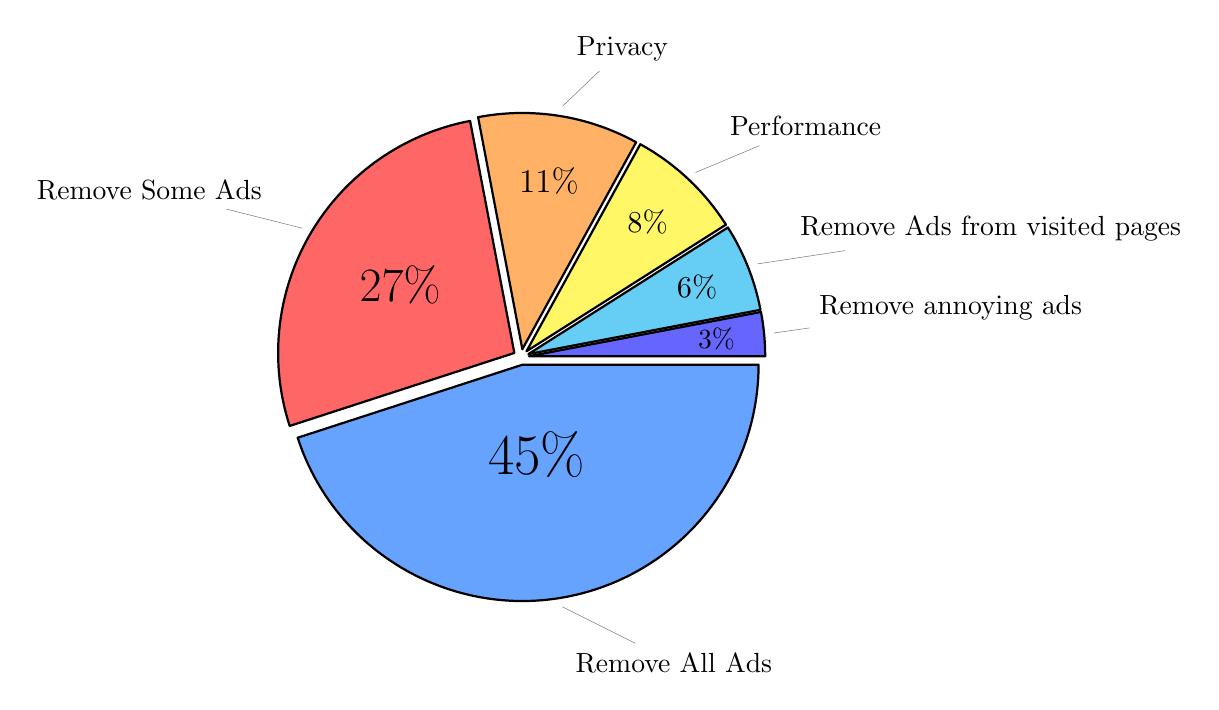
\begin{tikzpicture}
        \pie[ text = pin, scale font, pos ={8 ,0} , explode =0.1 ] {3/Remove annoying ads, 6/Remove Ads from visited pages, 8/Performance, 11/Privacy, 27/Remove Some Ads, 45/Remove All Ads}
    \end{tikzpicture}
        \caption{Survey results on questioning why users block ads \parencite{publishersWeb}.}
        \label{fig:adBlockingChart}
\end{figure}

% add graph from adobe pdf about why people block ads 
There are a multitude of reasons why a user may choose to block adverts Figure \ref{fig:adBlockingChart} illustrates a number of the most common. You can see that the largest proportion of the graph 45\% is users who wanted to remove all adverts from their browsing experience \parencite{publishersWeb}. The second largest segment 27\% of users wanted to remove ads they found especially annoying \parencite{publishersWeb}. Whilst others sighted privacy, performance and tracking as the reasons they wanted to remove adverts. Although Ad Blocking may pose a number of advantages for web users, it may be damaging not only to the advertising and connected industries but the entire web environment. \\

% discuss how this will effect web ecosystem (paywalls)
As technology develops and Ad Blocking becomes more commonplace, the growth in Ad Blocking usage may receive a sharp growth from mobile users,  this has the potential to challenge the viability of the web as a platform for the distribution of free ad-supported content \parencite{adobeAdBlock}. Although organisations such as Forbes have began to hide some content from users who are using Ad Blocking software whilst showing banners explaining they offer users a ``ad light'' version of the web page to encourage them to not use the Ad Blocking software, there is no guarantee that users will simply not move to the next content supplier who does not have such restrictions \parencite{publishersWeb}. Other organisations such as GQ have taken a different approach, asking users to disable their ad blocker to view their content or pay a small fee such as 50 cents per article \parencite{gq}.  This vicious cycle could see the end of the ``free web'' where information is supported via the use of adverts and in turn create an Internet littered with ``Paywalls'' where users must have a paid subscription to access content. Although Internet users may see some adverts as intrusive and annoying, the use of Ad Blocking software is having a detrimental effect on the web ecosystem which is so heavily reliant upon advertising. If a solution is found, that pleases both parties, such that users are no longer faced with intrusive and annoying adverts that impede their browsing, and content providers are still able to provide their content using the funding of ads then there may be some balance. However, if a solution is not found the content and knowledge of the web could be locked behind many paywalls which would be detrimental for all web users.

\pagebreak

\section{Online Advertising Fraud}
With the recent move to utilise Real Time Bidding platforms, online advertising fraud has become increasingly ubiquitous, due to the lack of human supervision within the process. Ad fraud can be defined as ``any time an impression or click is served to a non-human user (aka bot), or shown in an intentionally non-viewable inventory space" \parencite{dstillery}. There are numerous subsections of advertising fraud, this paper will focus on hidden ad impressions, paid traffic fraud and re-targeting fraud.   

%This happens via a process of fraudulent arbitrage, whereby fraudulent ad traders buy ad slots through one display ad exchange and then resell each of these ad slots multiple times through other display ad exchanges. Fraudulent ad traders achieve this by stuffing hidden webpages within the ad slots they buy. 

\subsection{Hidden ad impressions}
Hidden ad impressions sometimes referred to as ``Ad stacking" or ``Ad stuffing" is a method of fraud, in which advert impressions are hidden from the user, as they are simply to small for the human eye to recognise or placed in sections of the webpage that are not visible. For example, a study conducted by the security firm White Ops for the Association of National Advertisers (ANA) found as many as 85 adverts on a single page of which most were completely hidden to the user, as they were mostly 1x1 pixels in which an advert was served \parencite{botfraud2015}. Another method used to hide ad impressions is stacking the adverts on top of one another, such that the user of the web page will only see the advert at the top of the pile, however the web page will have served and be paid for multiple adverts. A 3D diagram of hidden ad impressions can be seen in Figure \ref{fig:ad_stacking_3d}, the orange adverts would be reported viewable by the browser although in reality they are hidden behind the green advert which is displayed in the foreground.  \\

This form of advertising not only applies to image adverts but also video adverts, which can be served in 1x1 frames and looped in sections so no user can see them. This form of advertising fraud can be used in tandem with click fraud to boost fraudulent revenue by artificially increasing the volume of clicks on adverts by utilising a botnet. This is typically utilised by a lower standard of inventory sources who are looking to increase their overall inventory revenue by making their page more attractive to potential advertiser with a higher click through rate.   \\

\begin{figure}[H]
    \centering
    \includegraphics[width=0.5\textwidth]{ad_stacking_3d.png}
    \caption{A 3D representation of ad stacking}
    \label{fig:ad_stacking_3d}
\end{figure}

Hidden ad impression fraud can have far-reaching consequences on advertisers, as millions of adverts can be sold on Ad Exchanges daily but none of these ads will ever be seen by a human user. The Interactive Advertising Bureau estimates that the direct costs of this fraud in combination with the lost revenue opportunity cost will cost the US marketing and media industry \$8.2 billion per year \parencite{iabfraud}. Although organisations are increasingly guarded about releasing information about their anti-fraud implementations for fear of losing their competitive advantage, there are numerous methods available to combat this method of fraud. For example, organisations such as Forensiq, ComScore and DoubleVeify offer services as fraud detection companies. Furthermore, accredited Ad Servers such as DoubleClick, Sizmek and Atlas Solutions all adhere to rigorous anti-fraud standards of either the Media Rating Council or the Interactive Advertising Bureau or both, each of these organisations use proprietary technology to watch for impression fraud. \\

Although purchased by Google in February 2014, Spider.io was one of the first organisations to explore ad visibility. An example of ad stacking can be seen in Figure \ref{fig:adstack}. Figure \ref{fig:legitAd} shows an Ad slot which is sold through one display Ad Exchange, this is typically a high quality webpage which would attract a human user. This is contrasted with Figure \ref{fig:adFraud}, which depicts a webpage filled with numerous adverts each of which will be sold immediately by the Ad trader through multiple display Ad Exchanges \parencite{spiderIo}. The Ads in Figure \ref{fig:adFraud} that are orange are adverts that when the position of the advert is inspected by applying simple geometry in relation to the browser window, would be incorrectly considered viewable, this is because the boundary of the browser window fully encloses the boundaries of the ad impressions \parencite{spiderIo}, however they are not viewable due to ad stacking as it is merely the top image in green which a user will see. The red adverts are outwith the viewable area of the browser window.  \\ 
% TODO: find a stat to back this up. Discuss figure

\begin{figure}[H]
    \begin{subfigure}{0.3\textwidth}
        \includegraphics[scale=0.3]{viewable_ad.png}
        \caption{A legitimate web page displaying one advert \parencite{spiderIo}}
        \label{fig:legitAd}
    \end{subfigure} \hspace{0.2\textwidth}
    \begin{subfigure}{0.3\textwidth}
        \includegraphics[scale=0.3]{fake_viewability.png}
        \caption{A web page displaying multiple adverts which are hidden to a user \parencite{spiderIo}}
        \label{fig:adFraud}
    \end{subfigure}
    \caption{A comparison of legitimate advertising and hidden ad impressions}
    \label{fig:adstack}
\end{figure}

Unfortunately, there is no silver bullet to completely remove ad impression fraud, there are a multitude of methodologies that can be utilised in conjunction with one another, to attempt to ensure that an advert is seen by a human use, however this is no guarantee. 

\subsection{Paid traffic fraud}
One of the largest challenges in the paradigm of online advertising is how to ensure human users are actually seeing and then clicking through adverts. Bloomberg reported that 11\% of display ads and 25\% of video ads placed on the Internet in 2014 were seen by bots, instead of human users \parencite{bloomFraud}. This correlates with the research of the Financial Times newspaper that found that part of a Mercedes-Benz on-line advertising campaign was viewed more often by computer bots than by real human users. With legitimate human users amassing only 43\% of the views \parencite{mercFraud}. \\

Advertising is suffering heavily from the prevalence of Bot Nets, which can be defined as a network of private computers infected with malicious software (malware)  and controlled as a group without the owners' knowledge. In the case of advertising fraud, bot nets are being used when publishers purchase traffic (views) for their website to help boost the price of their advertising inventory, as the more views a site has the higher the price it can demand for publishing adverts. Now that the purchasing of `fake traffic' is so ubiquitous in the advertising industry it has given rise to an industry of countermeasures \parencite{bloomFraud} where publishers are constantly battling the ever increasing number of fake or software related views. This will damage advertisers most, as they are forced to check whether their ads are being viewed by the ever increasing army of bots instead of potential human clients. The 2015 ``Bot Baseline: Fraud in Digital Advertising report" concluded that adverts viewed by non-human traffic will cost advertisers \$6.3 billion in 2015 \parencite{botfraud2015}, this figure is predicted to increase to \$7.2 billion in 2016 \parencite{botfraud2016}. This shows the prevalence and scale of advertising fraud and that advertisers and publishers must work together to help to mitigate the effects of the fake traffic associated with bot nets. \\

Publishers are currently using multiple methods to detect nonhuman traffic however, there is no single standard used by the industry. This form of fraudulent activity is the biggest threat to the online advertising industry. However, as long as publishers continue to buy traffic to their website for the purpose of boosting their advertising revenues, this fraudulent activity looks set to continue.

% TODO: Resarch this ADD more about retargeting cite image
\subsection{Retargeting Fraud}
Re-targeting fraud is the process in which bots can be programmed to mimic specific and highly desirable user behaviour, for example this could take the form of a bot pretending to have an interest in a specific brand of car, travelling to the relevant webpage and acting like a normal consumer intending to make a purchase. In depth behaviour may include, researching relevant topics on websites and clicking on ads, all without actually making a purchase. This behaviour then activates a campaign of re-targeted ads, which attempt to attract this potential customer to purchase the car, however the user was a bot. This may boost the revenues of a fraudulent publishing site by allowing it to demand the higher CPM associated with retargeting, on their page which the bot user will travel too. Figure \ref{fig:retargeting_fraud} displays the process of retargeting fraud. In step 1 the bot net visits a product webpage, in this example the product is an iPhone. Step 2 illustrates the heuristic research that the botnet will conduct visiting different related webpages and utilising search engines to investigate the product. Finally in step 3, the bot net will return to the web page owned by the bot net operator which will have ad impressions for sale which can now demand a much higher price due to the retargeting campaign which Apple (the product owner) will now be conducting to attract the customer to fulfil their purchase of an iPhone.  \\

\begin{figure} [H]
    \centering
    \includegraphics[width=1\textwidth]{retargeting_fraud.png}
    \caption{The re-targeting fraud process}
    \label{fig:retargeting_fraud}
\end{figure}

The ANA has a number of suggestions about how to combat Bot fraud especially in re-targeting campaigns, they suggest to use a form of third-party monitoring and bot detection to reveal bots within re-targeting campaigns and audience metrics, as this will prevent any further media being targeted at those bots, thus improving campaign metrics \parencite{botfraud2015}. A further recommendation is to apply day-parting where possible, as the ANA noticed a large proportion of bot fraud traffic between midnight and 7 a.m so advice to all entities is be vigilant during this time frame. Finally, updating of blacklists frequently and with precision is required to effectively block bots from viewing ads. For blacklists to be effective they must be updated at a minimum daily, and must be very specific to avoid blocking legitimate users \parencite{botfraud2015}.  

\pagebreak

\section{Requirements specification} \label{requirements}

\subsection{Primary}
The primary requirements for the project are detailed below:
\begin{itemize}
    \item Produce a browser extension to expose the Source and ID properties of IFrame advertisements in the context of the host page.
    \item Create clear documentation about the different entities and how they interact with one another during the targeted advertising process.
    \item Create a centralised resource containing information about all areas of targeted advertising.
    \item Provide a detailed account of the various methods of stateful tracking and stateless fingerprinting used to track and build profiles of users for the purpose of targeted advertising.
\end{itemize}

\subsection{Secondary}
The secondary requirements are as follows:
\begin{itemize}
    \item Produce a browser extension which exposes all IFrames on a page. Presenting the output in a readable manner including a count of the number of IFrames, search and copying functionality. 
    \item Discuss the effects of ``Ad Blocking". 
    \item Propose defences that a user could utilise to mitigate the effects of tracking and profiling.
    \item Create a glossary of frequently used terms in the online advertising industry.
\end{itemize}

\subsection{Tertiary}
\begin{itemize}
    \item Include a discussion of the various methods of advertising fraud.
    \item Discuss the future of tracking and profiling.
\end{itemize}

\section{Ethics}
Since this project does not use any personal or classified information and did not necessitate any experimental research involving human participants, this project does not raise any ethical concerns. 

\pagebreak

\section{Design}

\subsection{Design of IFrame Explorer}
For the implementation section of this project, I had envisaged with the support of my supervisor and an industry expert to create a browser extension which could be of use when exploring adverts displayed on a web-page.  \\

The extension would be used to detect advertising IFrames within a page and then overlay the HTML source of the IFrame object over the image of the advert. This idea can be seen below in a diagrammatic example in Figure \ref{fig:mockup}. 

\begin{figure}[H]
    \begin{subfigure}{0.3\textwidth}
        \includegraphics[scale=0.25]{siteWithAds.png}
        \caption{The web page displaying the images of an advert}
        \label{fig:siteWithAds}
    \end{subfigure} \hspace{0.2\textwidth}
    \begin{subfigure}{0.3\textwidth}
        \includegraphics[scale=0.25]{siteWithAdSource.png}
        \caption{The web page with the adverts source placed ontop of the advert}
        \label{fig:siteWithAdSource}
    \end{subfigure}
    \caption{The effect of the extension shown on a web page.}
    \label{fig:mockup}
\end{figure}

I chose to develop the extension for the Chrome browser, largely due to input from the industry expert as well as the usage statistics on web browsers that showed Google Chrome had the largest browser market share of 67.4\% in November 2015 \parencite{browserStats}. The Chrome extensions platform offers a wealth of APIs which would be of use throughout development. \\

\subsection{Design of iFetch}
Along with this extension I felt it was necessary to have a way for a user to view, search and copy the IFrames available on a web page. Therefore I designed a second extension, which would be used to display this information to the user. \\

I felt a popup window was the most suitable method to display this information to the user, therefore I planned that when a user pressed the browser action button a popup would display this information to the user, allowing them to both search and copy the information in case it required further processing. This can be seen diagrammatically in Figure \ref{fig:AE_Mockup}.

\begin{figure}[H]
    \centering
    \includegraphics[width=0.75\textwidth]{AE_Mockup.png}
    \caption{The iFetch extension showing the source of IFrames on a page}
    \label{fig:AE_Mockup}
\end{figure}

These tools were designed to be of use to both the industry expert and an everyday user. As they offer different functionality but complement one another they form the basis of an online advertising exploration framework. 

\subsection{Methodologies Utilised}
To ensure accountability and relevance throughout the development process, back-up copies of my work and notes on how well it was meeting the requirements defined by both my supervisor and the industry expert were maintained. Techniques from professional software development approaches and strict version control were used. \\

For general project management I created a Scrum Board which I used to delegate tasks relating to all areas of the development and reporting of the project. I split the project into three sections ``TODO" which could be formalised as the product backlog, ``In Progress" which included all tasks I was currently working on and ``Done" which included all tasks completed within the project. An example of the board during development can be seen in Figure \ref{fig:Project_Board}. This was a very useful tool throughout development as it allowed me to delegate my time as efficiently as possible, whilst ensuring that I had clear view on the goals and direction of the project for the entirety of the project.

\begin{figure}[H]
    \centering
    \includegraphics[width=0.5\textwidth]{Project_Board.png}
    \caption{A sample of the project board during development}
    \label{fig:Project_Board}
\end{figure}

 % TODO: Get screen shot of the user stories
During the requirements elicitation stage, I created numerous user stories from the perspective of a potential end user, this is in accordance with the Scrum methodology. I used the requirements defined in Section \ref{requirements} to form the basis of these stories whilst envisaging my supervisor and industry contact as potential clients that I was working for. I utilised the online task management platform \textit{Trello} to host my user stories and throughout the process I used the service to simulate my progression to achieving each story. A selection of user stories can be seen in Figure \ref{fig:sh_user_stories}.

\begin{figure}[H]
    \centering
    \includegraphics[width=0.60\textwidth]{sh_user_stories.png}
    \caption{User stories derived from the project requirements}
    \label{fig:sh_user_stories}
\end{figure}

Putting the requirements into terms of user stories helped to add a level of professionalism to my project as I did my utmost to ensure I completed the functionality of the user stories before progress meetings with my supervisor and the industry expert. These stories helped to keep me focused on the goals of the project throughout the development process whilst ensuring the development came in incremental stages. I used these progress meetings to get feedback from both my supervisor and the industry expert to improve the software as much as possible during the development stage of the project and to assure that I produced a deliverable which was desired by the industry expert and that met the requirements set out at the beginning of the project. \\

Throughout the project I set minor deadlines on the research that forms the basis of this report ensuring that I could submit draft copies to my supervisor and use his feedback to improve the research as much as possible. 

\subsection{Version Control}
To ensure I had a form of redundancy in case of a disaster scenario I used the distributed version control system Git to ensure the safety of my project's software. I used Git because I had a large amount of prior experience with the platform as I had used it throughout my university career but most specifically during the third year group project. I had considered using Mercurial, however I felt I was more accustom to Git and preferred it to Mercurial. I chose to manage my code base on a private GitHub repository, as Github offers the most informative and intuitive GUI for repository management. Although it could be argued that this was a risky decision, due to the fact that GitHub is a private company who could potentially remove their services at any time, whereas I could have used the schools Mercurial server. A vast majority of popular open source software is hosted on GitHub, for example the Linux Kernel, therefore the chances of this happening are very remote.  Also since Git is distributed by design if GitHub became unavailable, the local copy of the repository could easily be utilised to create a backup on another server, ensuring I never lose access to the code.

\subsection{Architecture of a Google Chrome Extension}
A Google chrome extension is a collection of files— HTML, CSS, JavaScript, JQuery, images, and anything else that adds functionality to the Google Chrome browser. There are numerous different browser extension user interfaces, both extensions developed for this project make use of the Browser Action interface, which allows a clickable icon to the right hand side of the address bar next to the menu bar which is represented as three horizontal bars. \\

A valid Google chrome extension must have a manifest file which is represented in JSON and may contain optional elements such as: HTML files, JavaScript files and any other files that extension may make use of such as images. \\

\begin{figure}[H]
    \centering
    \includegraphics[width=0.75\textwidth]{general_plugin_arch.png}
    \caption{Architecture of a Google Chrome Extension}
    \label{fig:general_plugin_arch}
\end{figure}

The manifest file, \textit{manifest.json}, is used to provide information to Google Chrome about the extension. Attributes that the manifest will provide information on is the name of extension, permissions required by the extension, a brief description of the extension and all optional files discussed previously. A high level representation of the architecture of a Google Chrome extnesion is shown in Figure \ref{fig:general_plugin_arch}. 

\subsection{Architecture of IFrame Explorer}
The first extension produced for this project contains a background page called \textit{background.js}. This is an invisible page running in the background which is utilised to set an \textit{onClickListener} for the browser action icon. Once this icon is clicked the extension will execute a JavaScript file and then in the callback function to this operation execute a further JavaScript file. The first script called \textit{jquery.js} is used to inject JQuery, the popular JavaScript library, into the current tab's page, then in the call back from this the script, \textit{iframe\_explorer.js}, containing the IFrame exploration logic is executed. \\

A content script, called \textit{highlight.js} is also utilised to perform the highlighting of the IFrame objects with a red border. Content scripts are run in the context of the host page for any page which matches the pattern defined in the manifest file. These files are discussed in more detail in Section \ref{Content_Scripts}. 

\subsection{Architecture of iFetch}
The second Google chrome extension created for this project is called iFetch and it is utilised to provide the source of all IFrame objects within a page in centralised searchable and easy to use manner. When clicked upon the popup displayed will detail all of the IFrames on a web page, these can then be searched using the search bar and if any IFrames exist the list of them can be copied, by using the copy icon, so that they can be utilised in another program. \\

This extension includes a script called \textit{popup2.js}. Which is run once the user clicks on the browser action icon and is utilised to handle the user initiated events such as the searching the IFrames within the page and copying the list of IFrames by clicking the copy icon. \\

Within the extension package, a file \textit{popup.html} exists which is the HTML page rendered by the extension when the user clicks the browser action button. This page is used to display the the list of the IFrames within the page, the search bar and the copy icon. When the browser action button is clicked, the popup web-page appears along with this, the script \textit{popup.js} is invoked. Once the current tab's web-page has loaded, this script will execute a further JavaScript file called \textit{getPageSource.js} which will gather the source of the current tab's webpage and return this via message passing between scripts for processing in the popup script. This information will then be displayed in a human readable manner to user, with both search and copying functionality available.

\pagebreak

% TODO: Add more design decisions
\section{Important Design Decisions}

\subsection{Content Scripts} \label{Content_Scripts}
% Content Scripts
The use of content scripts is crucial for the IFrame Explorer extension as they facilitate it to edit the current web page once it is loaded. By design content scripts run in the context of web pages loaded by the browser. Content scripts execute in a special environment called an ``isolated world". They have access to the DOM of the page they are injected into, but not to any JavaScript variables or functions created by the page. \\ 

A content script facilitated the extension to programmatically inject JavaScript into the browser loaded webpages, utilising the Google Chrome \textit{tabs.executeScript} API. The injected script utilises JQuery CSS functionality to highlight all IFrame objects with a red border and then to execute a script which on the click of the Browser Action button, will replace the IFrame advert with the objects id and src (source) attributes.  \\

% Security with content scripts
This process of inserting scripts may sound like a potential security flaw and as extensions may carry personal sensitive information there is a mechanism in place to ensure the safety of this data for extension users. The structure of the web pages Document Object Model (DOM) is shared between all scripts active on the webpage, e.g. scripts that have been placed on the web page by the owner, along with any scripts inserted into it by a content script. However each script operates in its own isolated world, which contains its own clean JavaScript environment which ensures that libraries and scripts do not conflict with one another. Many isolated worlds may operate on the same shared DOM tree but as security precaution they each get their own compliment of JavaScript objects to represent the tree. As no JavaScript objects are shared between these isolated worlds it is not possible for webpage scripts to use the shared DOM to become free of the normal web browser sandbox and somehow get access to the content script or any of the powerful APIs available to the extension. 

\subsection{Use of JQuery}
I chose to use the JavaScript library JQuery in this project as it is a fast and lightweight framework that facilitates easier HTML document traversal/manipulation and event handling than pure JavaScript. It also has an easy-to-use API with a small learning curve although its syntax is different to JavaScript, examples of the same functionality can be seen in JavaScript in Listing \ref{jsExample} and in JQuery in Listing \ref{jqExample}. As shown by the two examples, JQuery offers a much more concise version of the functionality and it also makes some processes such as changing the CSS attributes of an element much simpler than with traditional JavaScript. A further reason for choosing  JQuery is that it has been developed with cross-browser functionality at forefront of its  implementation, therefore in future if I looked to extend my project the source code would be highly portable to a variety of applications and web browsers. 

\begin{lstlisting}[caption=Setting the onClick functionality of button in JavaScript, label={jsExample}]
document.getElementById("button1").addEventListener("click", function(){ 
    alert("Hello");
});
\end{lstlisting}

\begin{lstlisting}[caption=Setting the onClick functionality of button in JQuery, label={jqExample}]
$("#button1").click(function(){ alert("Hello"); });
\end{lstlisting}

\pagebreak

\section{Implementation}

\subsection{IFrame Explorer}
It was difficult to develop the IFrame Explorer extension as numerous approaches I took to expose the source of the IFrames resulted in development being halted by security measures placed on the browser such as the Same Origin Policy and Cross-site scripting (XSS). Therefore a significant proportion of my development time was taken up by attempts to circumvent these security restrictions, until I found that they may be ignored by Content Scripts enabled within a Google Chrome extension. Even with content scripts finding a way to operate the JQuery library in the context of an extension whilst also injecting my script to perform the changes took a large amount of time. This process is complicated as it involves a bit of indirection such that the JQuery script must be executed first, so that the JQuery methods are avaliable in the second script, so that it can function as intended. Whilst this may seem relatively trivial after development, it is a bespoke problem in such that there was little documentation regrading how to go about this problem and it took up a large amount of my time to research and implement this functionality, with frequent trial and error approaches. \\

During development, I became aware that to place the IFrame attributes over the image of the advert lead to unclear results as the image attracted attention away from the attributes and in some cases obscured them completely. I therefore deviated slightly from design in that the extension replaces the IFrame image with its source attributes. Therefore the advert will be replaced with a red box including the IFrame source and id values. \\

Screenshots of the Express webpage \url{http://www.express.co.uk/} can be seen below Figure \ref{fig:express_before_no_plugin} shows the webpage with the extension disabled. This is contrasted with Figure \ref{fig:express_after_plugin} which illustrates the results of using the extension on the webpage. 

\begin{figure}[H]
    \centering
    \includegraphics[width=0.75\textwidth]{express_before_no_plugin.png}
    \caption{The web page displaying with the extension disabled}
    \label{fig:express_before_no_plugin}
\end{figure}

The numerous adverts on the webpage are replaced with the source attributes of the IFrames they belong to.

\begin{figure}[H]
    \centering
    \includegraphics[width=0.75\textwidth]{express_after_plugin.png}
    \caption{The web page after the use of the extension}
    \label{fig:express_after_plugin}
\end{figure}

\subsection{iFetch}
I began development of the iFetch extension by detailing the attributes of the IFrame objects in a centralised searchable manner via the popup page. As discussed in the design of this extension, I attempted to be as modular as possible, fitting each of the distinct areas of functionality into one JavaScript file, as I felt this would enhance the portability of the code as if I had to utilise the code in other areas of the project then this would be easily accomplished due to the loose coupling of the components. Once I had tested to ensure the IFrames were appearing correctly and in a readable manner, I began to implement the search functionality. The search function is a regular expression which is used to pattern match each of the IFrame objects to identify if any contain the user supplied search term, each IFrame that contains the term is then returned to the user and those that do not are omitted from the results. The copy functionality makes use of the \textit{document.execCommand} API, when the parameter ``copy" is passed into this function the text within a predefined area is copied to the user's clipboard. \\

The development of this section of the project largely went to schedule, although it did take me some time to familiar with the Google Chrome extension platform and some of the best practises when developing in this environment. Figure \ref{fig:iFetch_impl} shows the output of running iFetch on the \url{http://www.theguardian.com/uk}. There are 10 IFrames on the guardian page which could be searched, copied and inspected by a user of the extension. This method of interaction is much faster than a user having to open developer tools within their browser and trying to find each of the IFrames within the vast amount of source code a modern web page would have. This functionality is of strong use to those involved in the online advertising industry, including the industry expert's organisation, and user's who are interested where an IFrame originates from.     

\begin{figure}[H]
    \centering
    \includegraphics[width=0.75\textwidth]{iFetch_impl.png}
    \caption{Running iFetch on the guardian homepage}
    \label{fig:iFetch_impl}
\end{figure}

I achieved all of the requirements set out for this extension and the readable representation of the IFrame data is a novel approach to fetching the related source code of the web page. \\

The combination of both extensions will hopefully form the basis of a framework that users can benefit from, regardless of whether they are within the online advertising industry or external to the industry. In particular, the novel interface of the IFrame Explorer is something I am proud of as it replaces all the IFrames on a web page with their respective attributes with the click of one button. However, the extensions are not perfect and I have outlined my plans to improve them in the future in Section \ref{futureWork}.  

\subsection{Difficulties} \label{diff}
% Time to decide on deliverable
It took longer than expected to identify a potential deliverable for this project. This was largely  due to targeted advertising being a secretive and poorly documented area. Furthermore, I particularly wanted to create a deliverable that would add business value to my industry contact's organisation rather than re-creating something that exists already, I wanted to create something novel. This meant whilst conducting the research of this niche area, which forms the basis of this report, my supervisor and I were investigating  what could be of potential use in industry, this provided a significant development challenge for this project. \\

% Lack of documentation
There was a large number of development difficulties with this project, as there is a distinct lack of documentation regarding how to interact with advertising IFrames. This is largely due to the fact that online advertising is a secretive business as the revenues are largely dependent upon these IFrame adverts. Accordingly a significant amount of time throughout this project was spent researching and documenting potential approaches which may have achieved the aim to expose the source and id of IFrame objects via the means of a browser extension. The extension I produced is unique, to my knowledge there has never been a project to reveal the source of IFrames before. Due to the novel nature of the project and the lack of documentation in a majority of the areas development time was cut short due to disproportional amount of research which had to be conducted to understand the inner workings of online advertising. \\

% Web pages formatting Add a figure of a bad example 
A further difficulty when developing the IFrame Explorer extension, was the variety of formatting applied to webpages on the Internet. The web has become rich with a variety of formatting utilising both Cascading Style Sheets (CSS) and JavaScript. When trying to standardise my extension for the varying formats of these pages I found that I was often left with overlapping or obscured boxes due to the formatting of the host webpage. These formatting issues sometimes made the text unreadable when placed on the host webpage, although in most cases the text could be seen and copied even if a small section was obscured by elements of the host page. An example of this can be seen in Figure \ref{fig:ie_overlap_diff}, whilst the text of this IFrame box is visibly obscured the text can still be highlighted and copied by the user, using right-click copy functionality. This has the knock on effect that my extension works effectively on a large range of web pages however due to the formatting on others its functionality is infrequently inhibited. I tried numerous methods to help detect this poor formatting, however they did not significantly improve the positioning of the exposed IFrame objects. This is a general problem of developing applications for the Internet, in that it may work in a majority of cases but not in every. I wanted the position of the IFrames to remain largely relative to where they were before use of the extension, to ensure the user gets a better idea of the position of the objects in relation to the host page. So to ensure that they are always visible, do not overlap and remain in the original position is all but impossible. However,  in the future, I would look to improve this by a form of compromise, which will show the position of overlapping frames and attempt to keep all information within the IFrame boxes visible. \\

\begin{figure}[H]
    \centering
    \includegraphics[width=0.75\textwidth]{ie_overlap_diff.png}
    \caption{An IFrame box is hidden slightly behind an image}
    \label{fig:ie_overlap_diff}
\end{figure}

I would have liked to extend both extensions further offering more functionality, however this was not possible given the time scale of the project and difficulties discussed within this section. The main areas in which I would like to extend the project in discussed in Section \ref{futureWork}.

\pagebreak

\section{Testing}
Unlike a traditional program which may prove its desired functionality via extensive unit testing and potentially formal verification. These approaches do not lend themselves easily to testing a browser extension which is concerned with implementing changes to appearance of a host webpage. I felt that these forms of testing should be secondary to usability testing of the extension. Thus, I decided to separate the testing into two distinct areas, firstly I created a testbed on my school host server, which I used throughout development to ensure the requirements of the extensions were met. Secondly, I carried out numerous tests on popular web pages on the Internet to see how well the extensions would scale in a real world use case. 

\subsection{Testing IFrame Explorer}

\subsubsection{Testbed}
I have created an online webpage which has information about the IFrame Exploration extension and can be used as a local testbed to demonstrate the functionality of the extension. I created this to showcase the functionality of the extension and to ensure a repeatable testing process that a marker could utilise. The testbed can be found at the following URL: 

\begin{center}
\url{https://ms255.host.cs.st-andrews.ac.uk/SH/index.html}
\end{center}

This was created to simulate an online news article and has numerous IFrame advert images inserted around the article. When a user has the extension installed they can use it to reveal the source of the images and see the potential use case for the browser extension. Details of how to install a Google Chrome extension can be found in Section \ref{installPlugin} or from Google Chrome development webpage \url{https://developer.chrome.com/extensions/getstarted#unpacked}. Instructions on how to use the extension can be found in Section \ref{userGuide}. The section of the webpage that allows simulation is titled Testbed. 

\subsubsection{In the wild} \label{ieWild}
I have used the extension in a wide variety of webpages across the Internet to gain an idea of its functionality and any potential areas of its functionality which may require improvement. Images of this testing can be found in the \textit{images} directory of the project. The results of this testing are compiled in Table \ref{table:2}. \textbf{Note} some webpages URLs were excessively long, therefore I used the URL shortening service of \url{https://bitly.com/} to compress them for a viewable format in the table. The extension performance column of the table is an absolute category rating scale as follows: Bad, Poor, Fair, Good, Excellent. The notes column also will contain any exceptional behaviour which will be further discussed in Section \ref{testSummary}. All of the data within Table \ref{table:2} was collected on 23/03/16, as discussed in Section \ref{diff} the changing nature and format of these webpages may alter the performance of the extension. \\

{
\begin{table} [H]
\centering
% TODO Table: 
\begin{tabular}{ |p{5cm}|p{5cm}|p{5cm}|  }
\hline
\multicolumn{3}{|c|}{\textbf{Internet Testing Results of IFrame Explorer}} \\
\hline
\textbf{URL} & \textbf{extension Performance} & \textbf{Notes} \\
\hline
\url{www.theguardian.com/uk} & Good & Overlap Menu bar \\
\hline
\url{www.independent.co.uk} & Fair & Box hidden behind menu bar \\
\hline
\url{www.express.co.uk} & Excellent & Great performance \\
\hline
\url{www.arstechnica.co.uk} & Poor & Box almost hidden completely by menu bar  \\
\hline
\url{bit.ly/1LRt8Vh} & Excellent & Great performance but font does not change colour \\
\hline
\url{www.telegraph.co.uk/news} & Excellent & Great performance   \\
\hline
\end{tabular}
\caption{Table shows results of using the IFrame Explorer extension on Internet webpages. The potential scores are: Bad, Poor, Fair, Good, Excellent}
\label{table:2}
\end{table}
}

A more detailed testing table can be found in the Testing Summary Appendix in Section \ref{iETesting}. The results of the entire testing process are summarised in the Figure \ref{fig:iePie}. This shows that the majority of the test runs, 58\%, resulted in a positive assessment either Good or Excellent. Whilst nearly a quarter of the test runs, 24.9\%, resulted in a negative assessment either Poor or Bad. The slightly high percentage of negative results can be attributed to the formatting issues discussed in Section \ref{diff}, which I would look to amend as future work. 

\begin{figure} [H]
    \centering
    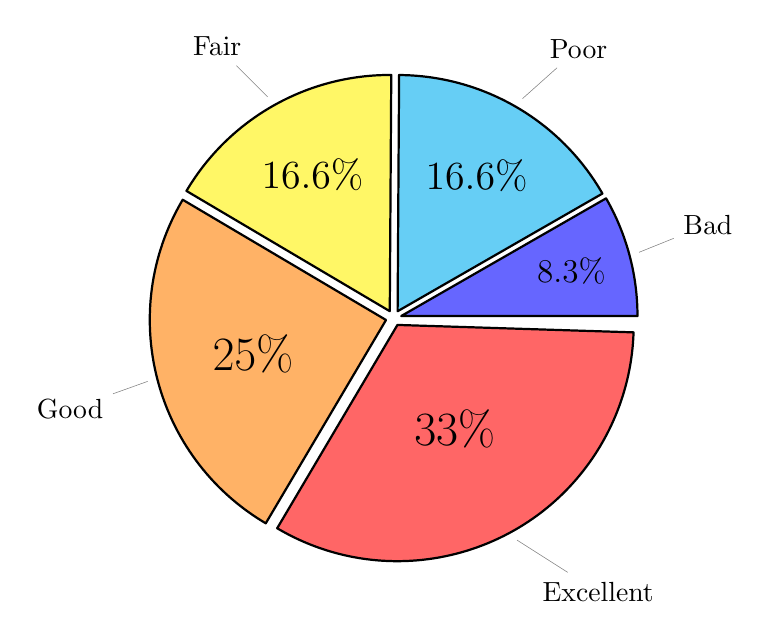
\begin{tikzpicture}
        \pie[ text = pin, scale font, pos ={8 ,0} , explode =0.1 ] {8.3/Bad, 16.6/Poor, 16.6/Fair, 25/Good, 33/Excellent}
    \end{tikzpicture}
        \caption{Summary of the IFrame Explorer testing results in the form of a pie chart}
        \label{fig:iePie}
\end{figure}


Within the Extension section of the testbed on my host server there is a gallery of before and after the use of the extension screenshots. A number of these can also be found in the images directory of the project deliverable. 

\subsection{Testing iFetch}
In a similar procedure to testing the IFrame explorer extension I used the testbed on my host server to form the basis of my testing during development of the iFetch extension. The extension can still be tested on the testbed it should count 5 IFrame objects 4 of which correspond to the adverts placed around the mock article and one which contains the video player. Once I was satisfied with the performance of the iFetch extension I began to test it on Internet webpages to identify any bugs and test the scalability of the source fetching functionality of the extension. An example screenshot of the testing process can be seen in Figure \ref{fig:iFetch_screen}.  

\begin{figure}[H]
    \centering
    \includegraphics[width=0.75\textwidth]{iFetch_screen.png}
    \caption{Using the iFetch extension on the ars technica webpage}
    \label{fig:iFetch_screen}
\end{figure}

Table \ref{table:3} shows the results of this testing. The measurement criteria used was a comparison between the number of IFrames identified by my extension, a manual inspection of the HTML source code of the webpage and visually inspecting the webpage. To gain the source code of the webpage I used the ``Developer Tools" of the Google Chrome browser, I then searched through the HTML identifying any IFrame objects. The results of this testing may not stay consistent with future runs as webpage owners increase or decrease the number of IFrames on their site. In future it would be interesting to contrast the number of IFrames presented on a page on a temporal and per user basis to identify any potential correlations. I had looked to automate this process via using a simple Python web scraping script. Unfortunately, the majority of the IFrames are loaded programatically by JavaScript thus, a traditional web scraping script would not return a full set of results. Therefore, the process had to be conducted manually and was time consuming. \\

The second column of Table \ref{table:3} represents the number of IFrames I identified when manually inspecting the HTML source code of the webpage. Column 3 presents the number of IFrames that I visually identified on the webpage, including advertising IFrames, social media buttons or video players. The final column presents the total number of IFrames found by the iFetch extension.    

{
\begin{table} [H]
\centering
% TODO Table: 
\begin{tabular}{ |p{4cm}|p{3cm}|p{3cm}| p{3cm} | }
\hline
\multicolumn{4}{|c|}{\textbf{Internet Testing Results of iFetch}} \\
\hline
\textbf{URL} & \textbf{Number of IFrames in page source} & \textbf{Number of IFrames viewable on page} & \textbf{Number of IFrames found by iFetch} \\
\hline
\url{www.theguardian.com/uk} & 9 & 5 & 9 \\
\hline
\url{www.independent.co.uk} & 26 & 10 & 26 \\
\hline
\url{www.express.co.uk} & 14 & 5 & 12 \\
\hline
\url{www.arstechnica.co.uk} & 15 & 3 & 10  \\
\hline
\url{bit.ly/1LRt8Vh} & 11 & 2 & 11 \\
\hline
\url{www.telegraph.co.uk/news} & 16 & 2 & 16\\
\hline
\end{tabular}
\caption{Table shows results of using the iFetch extension on Internet webpagess.}
\label{table:3}
\end{table}
}

The results of testing were interesting and fully depicts the difficulties of operating in an area as fast changing as targeted advertising. The majority of the results showed that iFetch returned the same number of IFrames as were identified in the source code inspection. However for a number of the pages more were identified in the source than were returned from iFetch. After a large amount of research into this fault I could not identify what was causing this issue, my hypothesis was that it could potentially be the nesting of IFrames which means that the source fetching function of the iFetch returns the top level IFrame without iterating through its contents to find lower level frames. However, having tested this hypothesis on my host server, iFetch returns the correct number when nested IFrames are used in this scenario. This is one of the largest complications of developing a program for usage with Internet sites is creating a reliable testing setup that fully recreates the environment expected in the wild on the Internet. In the future I would attempt to fully identify the root of this problem and amend it. However, in the majority of cases the extension returns the number expected. The full testing table can be found in Table \ref{table:5} in the Testing Summary in Section \ref{iFetchTesting}. \\

Figure \ref{fig:ifPie} shows the results of the testing process presented as a pie chart. The larger proportion of cases 66.67\% indictaes when the number of IFrames returned by iFetch matched the number of IFrames in the page source. Whilst, the smaller section of the chart 33.33\% indicates when the numbers did not match, which was due to more IFrames being identified during the source code inspection. As shown by the chart, largely the the extension functioned as required, although further work must be conducted to identify the why on some pages there is inconsistencies.  

\begin{figure} [H]
    \centering
    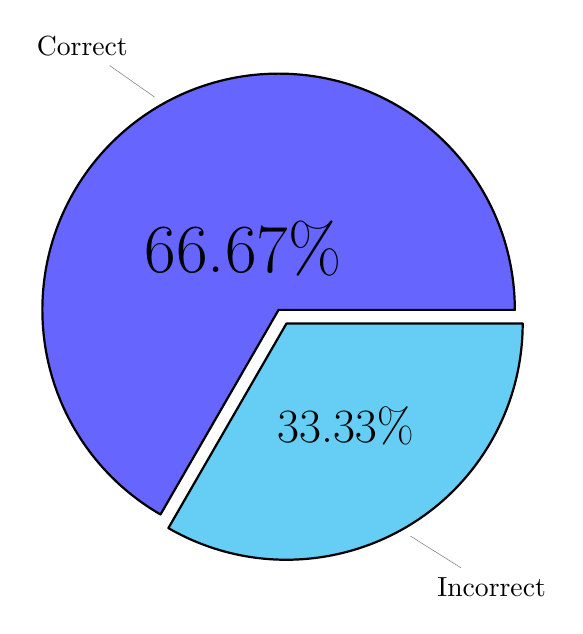
\begin{tikzpicture}
        \pie[ text = pin, scale font, pos ={8 ,0} , explode =0.1 ] {66.67/Correct, 33.33/Incorrect}
    \end{tikzpicture}
        \caption{Summary of the iFetch testing results in the form of a pie chart}
        \label{fig:ifPie}
\end{figure}

A further result of testing was that the number of IFrames viewable on the page was always significantly less than the number returned by iFetch this adds further validity to the hypothesis that a large proportion of IFrames on webpages are hidden IFrames which are present in the source code of the HTML but are not viewable by the user browsing the webpage. This would be an interesting topic for future research, as hidden IFrames which can be utilised for numerous legitimate reasons such as monitoring the success of advertising campaigns or they can be utilised for third party tracking and nefariously used for installation of malware and/or invisibly running scripts on pages, so to identify the number of hidden IFrames may have potential security benefits. 

\pagebreak

\section{Future Work} \label{futureWork}
% Article with Colin
In the future I will look to have a summary of the research of this report presented in the form of a journal article. My supervisor suggested that after the end of the current academic year we could begin drafting the article and this may involve some input from the industry expert. \\

% Improvement to the extension
I would like to improve the functionality of the IFrame Explorer extension to ensure that it can it can deal with overlapping IFrames and that all of its ouput is human readable. This would require a large amount of time and extensive testing on a large number of Internet web pages. It would also be on the presumption that these webpages do not change their formatting. However I feel it would make the extension significantly more useful and it may allow it to help to detect IFrame stacking fraud in conjunction with other tools that are available. Improved functionality for highly formatted webpages could be achieved by creating a template which is designed specifically for use on one site. The template would be based on the formatting of this site, then when the extension is executed on this webpage the template would be utilised to inform the positioning of the IFrame source attributes within this web site. To look even further to the future the task of developing these templates could be delegated to an employee of the organisation which the industry expert works for which would allow them to change easily whenever a page updates its formatting. \\

% Javascript placeholder bug
It is possible to load an IFrame object onto a webpage with no source specified and then later apply content to the IFrame object using JavaScript. This was an area which was unknown to the industry expert and I before we decided to create the deliverable. This effects the performance of the IFrame Explorer extension as it results in it displaying the src of an object as \textit{javascript:``"} or sometimes developers have used the cross browser placeholder of \textit{about:blank}. In the future I would look to see if it is possible to find out which JavaScript file set the content of the IFrame and return the name of this script to the user instead of this non descriptive placeholder. \\

% Fix iFetch bug
As mentioned during the testing section of the iFetch extension it sometimes produces inconsistent results when compared to manually inspecting the source code of the web page. Having thoroughly inspected this erroneous behaviour I have still not identified the cause and therefore in the future I would like to find the cause and resolve this issue. This would require a large amount of testing on the Internet as the issues appears to happen sporadically on some webapges on the Internet and not others (including my host server). The bug does not limit the functionality of the extension greatly as previously mentioned it is limited to a small proportion of sites and the efficiency boost granted when using the plugin for the industry expert's organisation would outweigh the inconvenience of occasionally having to use the tool as starting point and then returning to the previous method of manual inspection of the web page. \\  

% More attractive UI of iFetch / IFrame explorer
Although the user interface of the iFetch extension is acceptable if more time was afforded to this project I would liked to have improved the formatting of the popup page by adding a more attractive theme via CSS. This would not impact the functionality of the extension, it would only make it more aesthetically pleasing. However, for an application that is largely visual I think this is an important improvement that could be made. \\

Finally if more time was available for this project I would like to test the extensions on a much wider sample of Internet sites, as this would illustrate the scalability of the extension and would identify further areas which require improvement. A good sample to utilise would be the Alexa Top 500 Global sites \url{http://www.alexa.com/topsites}, as these are the 500 most popular webpages on the Internet and are commonly used for testing purposes in research.  

\pagebreak

\section{Evaluation and critical appraisal}
I have met all of the original objectives of my project. It has been difficult at times to meet these aims, however with a large amount of perseverance and research I have developed two extensions which meet the aims of both my project and the industry expert. Had there been more time available for the project I would have liked to have further extended it by meeting the criteria specified within Section \ref{futureWork}, however I feel that as a whole the project has been a success. It has brought to light numerous tactics employed by advertising organisations to track and eventually profile users. Whilst proposing some potential defences to these methods, along with a list of practical advice which could be utilised to limit the effects of tracking from a user's perspective. It has also produced two bespoke extensions which were requested by an industry expert as a means to facilitate faster access to IFrame source and ID attributes. The one area of the project could potentially require improvement is the placement of the IFrame source information on a webpage although as previously mentioned this would require much more time than is afforded to a project of this size. \\

I feel as though I took a risk by choosing a project that was based in such a secretive and volatile area, however, the benefits have been far-reaching from improving my own knowledge, producing a summary of research in the targeted advertising sector and creating a unique deliverable which met the requirements of the project and an industry expert. The deliverable is a prototype which would ideally be extended by the development team of the industry experts' organisation. The online advertising sector is an area which captivates me and is extremely contemporary as stories related to it reach the news on a weekly basis. It is a somewhat overlooked area as many users will see and interact with adverts but few truly know how the adverts arrive to their browser. This is what I hope my project can expose. \\

% other work done in area (research)
There has been considerable research in the online advertising industry, but for such an omnipresent and unstable area there is a lack of consolidation of this research. This project does not seek to compare with other research projects it looks to combine all of this wide ranging knowledge into one concise document from which users with a lack of technical knowledge can understand the techniques used in the online advertising industry. For example papers such as the ``Cookieless monster" which concentrated on methods to track users without traditional cookies \parencite{cookielessMonster}, the ``The web never forgets" article which focuses on all tracking mechanisms existent on the web today \parencite{webNeverForgets}, along with the ``Privacy regulation and online advertising" paper \parencite{goldfarb2011privacy}, have focused on the potential privacy invasion that tracking methods impose. There is little research conducted into finding which organisations are actively monitoring users and for what reason. This would be an interesting avenue to explore in the future.  \\

% other work publicly available tools
There are numerous tools available that will block adverts from appearing on a webpage ``ad-blockers" or tools that will help to prevent a user from being tracked. But the IFrame exploration tools looks to dig deeper, it is the first step to finding out where adverts are being served from and in correlation who may be tracking a user. 

\pagebreak

\section{Future of Tracking}
With the introduction of mobile-content blockers we have reached a pivotal time in the evolution of the World Wide Web. Desktop ad-blocking mechanisms have been around for a number of the years and are primarily concerned with enhancing privacy. For mobile devices however the other advantages are also highly important. For example bandwidth cost savings (a key issue for mobile data contracts) and faster page load times are crucial for the effective use of mobile web browsing. Whilst a key issue on desktop environments the privacy gain from the lack of tracking is simply a bonus. As the shift from traditional desktop browsing inexorably moves to smartphones losing the ability to target advertising to iOS could become a catalyst for a change in the free content available on the web \parencite{tippingPoint}. These technologies will deeply affect not only digital advertising and its related parties but also the entire web ecosystem. \\

The future of web tracking and targeted advertising is a shift away from the traditional methods of third-party cookies and JavaScript snippets, as these methods can no longer produce reliable results. The focus will shift to stateless tracking mechanisms such as the various forms of fingerprinting, which have been discussed in detail within this paper. The impact of an increase in privacy conscious users online privacy is likely to force organisations to adapt and find other ways to track and share data about users. For example Facebook has already introduced an approach called ``Custom Audience  Targeting" (\url{http://on.fb.me/1SnIX7x}) which can be utilised by advertisers to target adverts on Facebook to users whom they have already collected data from. As users become more technologically advanced in their blocking mechanisms techniques including ``universal IDs and IP reconciliation will also become more widespread and important to marketers and content platforms" \parencite{tippingPoint}. \\

Without the ability to reach users with advertising on their sites a lot of free-content on web pages may become hidden behind paywalls which are required to ensure the financial viability of web pages. If the Do Not Track (DNT) header had been implemented by governments  and advertising agencies there may not have been an issue with advert blocking however as long as there is a form of ad re-targeting where adverts follow user's around on third party pages this war between privacy and free content will continue. This is the tipping point where advertising organisations must begin to re-think their strategies and remove potentially annoying adverts and insidious tracking mechanisms and become more responsible. 

\pagebreak

\section{Conclusions}
% project is at the forefront of the debate over free content on the Internet and this debate may have massive consequences for all Internet users and the knowledge that is stored within web pages. 
This project is at the forefront of a volatile and secretive industry, its results can be used to fuel further research into where online adverts come from, why these companies are tracking users and how they created a profile for a user. The deliverable produced acts as prototype which can be extended to begin to identify which organisations are placing adverts within a page. The project is at the front line of the debate over free content on the Internet and this debate may have massive consequences for all Internet users and the knowledge that is stored within web pages. \\

Ultimately the web ecosystem is complicated and diverse. The war between online privacy and tracking will continue for as long as web users access content published on web pages supported by online advertising. The dependency upon advertising to fund the ``Free web'' has created an environment over-reliant on advertising to support itself. The ecosystem is over populated with ubiquitous intrusive tracking and advertising, even when privacy conscious users attempt to avoid these types of monitoring, techniques such as browser fingerprinting make it impossible for web users to avoid some form of profiling. This paper has delved into the various areas used to generate targeted advertising, attempting to bring these techniques to the forefront to expose them to users so they may be combated to return privacy to the hands of the users. \\

However, the genie is effectively out of the bottle; returning privacy to the hands of the users would require combined pressure from governments, standards organisations and web users which is unlikely to happen. An alternative model to the ``Free web'' in terms of advertising would be ``paywalls'' were information on web pages is only displayed to paying customers, which would create a fractured ecosystem where only users with enough money would be able to access the vast amount of information available on the Internet which is an outcome that would be detrimental for society as a whole. \\

In comparison to the wealth of information and free content available on the web, targeted advertising is a small price to pay. Personally, I feel that users would feel much more comfortable with the process if it was made more transparent by organisations explaining how their tracking procedure is conducted and allowing users to potentially opt-out. To conclude, whilst the techniques used to generate targeted advertising are insidious, the majority of adverts on the web do not impede web usage, these adverts underpin the majority of the free content on the web so are ultimately beneficial for almost all users of the Internet.

\section{Appendix A: Testing summary} \label{testSummary}

\subsection{IFrame Explorer Testing Table}  \label{iETesting}
Table \ref{table:4} below shows the performance of the IFrame Explorer extension on a wide range of popular Internet sites. All of the issues in the Notes column relate to formatting or styling issues. In the Sky Sports and Yahoo webpages the boxes for the IFrames were too small such that they looked like a single red line, however with the use of developer tools I could see the correct information of the advert was being displayed within the box and that it was merely a formatting bug which was stopping it from displaying correctly. These formatting errors are my number one priority to improve the extension in any future work. 

{
\begin{table} [H]
\centering
% TODO Table: 
\begin{tabular}{ |p{5cm}|p{5cm}|p{5cm}|  }
\hline
\multicolumn{3}{|c|}{\textbf{Internet Testing Results of IFrame Explorer}} \\
\hline
\textbf{URL} & \textbf{extension Performance} & \textbf{Notes} \\
\hline
\url{www.theguardian.com/uk} & Good & Overlap Menu bar \\
\hline
\url{www.independent.co.uk} & Fair & Box hidden behind menu bar \\
\hline
\url{www.express.co.uk} & Excellent & Great performance \\
\hline
\url{www.arstechnica.co.uk} & Poor & Box almost hidden completely by menu bar  \\
\hline
\url{bit.ly/1LRt8Vh} & Excellent & Great performance but font does not change colour \\
\hline
\url{www.telegraph.co.uk/news} & Excellent & Great performance   \\
\hline
\url{http://metro.co.uk/} & Good & Text in IFrames is too small \\
\hline
\url{http://www.amazon.co.uk/} & Excellent & Great performance but Amazon has few ads  \\
\hline
\url{https://www.washingtonpost.com/} & Fair & Text in IFrames is too big \\
\hline
\url{http://www.skysports.com/} & Bad & Some frames too small \\
\hline
\url{https://uk.yahoo.com/?p=us} & Poor & Similar functionality to sky sports \\
\hline
\url{http://www.imdb.com/} & Good & Minor formatting issues \\
\hline
\end{tabular}
\caption{Table shows results of using the IFrame Explorer extension on Internet webpages. The potential scores are: Bad, Poor, Fair, Good, Excellent}
\label{table:4}
\end{table}
}

\subsection{iFetch Testing Table} \label{iFetchTesting}
A detailed table below shows the performance of the iFetch extension on a wide range of popular Internet sites. 

{
\begin{table} [H]
\centering
% TODO Table: 
\begin{tabular}{ |p{4cm}|p{3cm}|p{3cm}| p{3cm} | }
\hline
\multicolumn{4}{|c|}{\textbf{Internet Testing Results of iFetch}} \\
\hline
\textbf{URL} & \textbf{Number of IFrames in page source} & \textbf{Number of IFrames viewable on page} & \textbf{Number of IFrames found by iFetch} \\
\hline
\url{www.theguardian.com/uk} & 9 & 5 & 9 \\
\hline
\url{www.independent.co.uk} & 26 & 10 & 26 \\
\hline
\url{www.express.co.uk} & 14 & 5 & 12 \\
\hline
\url{www.arstechnica.co.uk} & 15 & 3 & 10  \\
\hline
\url{bit.ly/1LRt8Vh} & 11 & 2 & 11 \\
\hline
\url{www.telegraph.co.uk/news} & 16 & 2 & 16\\
\hline
\url{http://metro.co.uk/} & 14 & 1 & 14 \\
\hline
\url{http://www.amazon.co.uk/} & 4 & 2 & 4 \\
\hline
\url{https://www.washingtonpost.com/} & 12 & 1 & 12 \\
\hline
\url{http://www.skysports.com/} & 12 & 2 & 10\\
\hline
\url{https://uk.yahoo.com/?p=us} & 7 & 3 & 7 \\
\hline
\url{http://www.imdb.com/} & 7 & 5 & 7 \\
\hline
\end{tabular}
\caption{Table shows results of using the iFetch extension on Internet webpagess.}
\label{table:5}
\end{table}
}

\section{Appendix C: User manual} \label{userman}

\subsection{Installing a extension} \label{installPlugin}
To install an extension in Google Chrome follow the steps below. Note a box with a red border in an image indicates the option to select. 

\begin{enumerate}
    \item Open the Google Chrome browser, and click the three horizontal bars menu. Select the \textbf{Settings} option. 
    
    \begin{figure}[H]
        \centering
        \includegraphics[width=0.75\textwidth]{chrome_setup_settings.png}
        \caption{The settings option is highlighted in blue}
        \label{fig:chrome_setup_settings}
    \end{figure}
    
    \item From within this menu select the \textbf{Extensions} option on the left hand menu.
    
    \begin{figure}[H]
        \centering
        \includegraphics[width=0.75\textwidth]{settings_b4_ext.png}
        \caption{The settings button is highlighted with a red box}
        \label{fig:settings_before_ext}
    \end{figure}

    
    \item In the extensions tab, ensure that the \textbf{Developer mode} option is ticked. 
    \item Click the \textbf{Load unpacked extension...} button
    
    \begin{figure}[H]
        \centering
        \includegraphics[width=0.75\textwidth]{extensions.png}
        \caption{Both the developer and load unpacked extensions options are highlighted with a red box}
        \label{fig:extensions}
    \end{figure}
    
    \begin{enumerate}
        \item In the popup menu, select the directory which contains the extension e.g. IFrame Explorer or iFetch. 
        \item The extension should then appear including its title and a brief description of its function.
        
        \begin{figure}[H]
            \centering
            \includegraphics[width=0.75\textwidth]{extensions_installed.png}
            \caption{Both of the extensions loaded}
            \label{fig:extensions_installed}
        \end{figure}
        
    \end{enumerate}
\end{enumerate}

\subsection{How to use the extensions} \label{userGuide}
Both extensions have a simple and intuitive User Interface (UI). They each have a Browser Action icon, which is placed to the upper right corner of the Google Chrome Browser next to the Menu button, this is shown in Figure \ref{fig:logos}. Upon pressing these icons the functionality of the relevant extension will execute. \textbf{Note} the IFrame Explorer will replace the content of the IFrame objects with its source attributes therefore they will no longer be on the page if you execute the iFetch extension. Therefore, if you want to check the number of IFrames or their source execute the iFetch extension before the IFrame explorer.  

\begin{figure}[H]
    \centering
    \includegraphics[width=0.25\textwidth]{logos.png}
    \caption{The logos of both extensions}
    \label{fig:logos}
\end{figure}

\subsection{Online Testbed}
The online testbed can be accessed from the following URL: 
\begin{center}
\url{https://ms255.host.cs.st-andrews.ac.uk/SH/index.html}
\end{center}

\section{Appendix D: Glossary} \label{glossary}

\subsection{Online Advertising}
Online advertising can be defined as any method of marketing that utilises the Internet as the vehicle to deliver the promotional content to the user. This is a very broad category which includes; email marketing, Search Engine Marketing (SEM), social media marketing and display advertising. Like traditional forms of advertising, online advertising will involve a publisher and advertiser. 

\subsection{Display Advertising}
Display advertising is advertising on web sites. It can involve many different formats and contains items such as text, images, video, and audio. The goal of this form of advertising is to deliver a general brand message to the visitors of the site,

% TODO: Concise def
\subsection{Targeted Advertising}
Targeted advertising is a form of advertising whereby advertisements are placed to attempt to reach consumers based on various traits such as demographics, purchase history, or observed behaviour. Numerous tracking methods can be used to improve the effectiveness of advertising such as cookies. 

\subsection{Behavioural Targeting}
Behavioural targeting utilises a range of technologies and techniques in combination to attempt to increase the effectiveness of advertising to benefit both advertisers and publishers. Most frequently, behavioural targeting uses information collected from an individual’s web-browsing behaviour, including their browsing history and searches on a search engine, to select advertisements to display. 

% TODO: Research this
\subsection{Behavioural Re-targeting}
Adverts are a fundamental part of the web ecosystem. Users have begun to expect adverts for the latest line of sports trainers, whilst they are browsing the web site of an online clothes retailer. However, whilst surfing the Internet users are becoming increasingly aware of ``behavioural re-targeting'' where an advert which may have been viewed on a completely different web site seemingly ``follows'' that user as they visit other unrelated web pages. This process is becoming increasingly prevalent as shown by a study of cookies in the top 100 web sites, in which an average of 57 cookies per web page was recorded, whilst 20\% of pages visited contained 100 or more cookies \parencite{taOffer}. However, the most concerning fact about this discovery was that 87\% of cookies on these web sites were set by third-parties \parencite{taOffer}. This is where the re-targeting process begins. Whenever the user visits a page within the same Ad Network (discussed in detail in Section \ref{AdNetwork}) the previous advert can be displayed to the user.

\subsection{Cost Per Mille (CPM) or Cost Per Thousand (CPT)} \label{cpm}
Cost Per Mille (CPM) is a commonly used measurement in traditional advertising mediums such as radio, television and newspaper. CPM refers to the cost or expense incurred for every thousand potential customers who view the advertisement. The terms Cost Per Mille and Cost Per Thousand are synonymous as in Latin mille means thousand. 

\subsection{Cost Per Impression (CPI)}
Cost Per Impression (CPI) is a statistic used in digital advertising where advertisers pay each time an ad is displayed. CPI is the cost incurred for each potential customer who views the advertisement.

\subsection{Click Fraud}
Click fraud is a type of fraud that occurs in pay-per-click (PPC) online advertising when a person, automated script or computer program imitates a legitimate user by clicking on an ad, for the purpose of generating a charge per click without having actual interest in the advertised product.

\subsection{Interactive Advertising Bureau (IAB)}
The Interactive Advertising Bureau is a non-profit organisation established in 1996, with a headquarters in New York, USA. The aim of the organisation is to develop industry standards, conduct research, and provides legal support for the online advertising industry. The core principles of the IAB is to: defend advertising organisations from adverse legislation and regulation; improve customer relationships to reduce friction in the supply chain; share best practises that foster industry-wide growth and conduct and publish research for the benefit of the advertising industry.

\subsection{ Internet Advertising Bureau (IAB UK)}
The Internet Advertising Bureau is a trade association (industry trade group) founded and funded by businesses that operate in the advertising industry. The IAB UK follows similar principles to the Interactive Advertising Bureau, to promote a strong and competitive digital advertising industry whilst promoting an environment to ensure digital advertising thrives. 

\medskip
\printbibliography

\end{document}